%% ODER: format ==         = "\mathrel{==}"
%% ODER: format /=         = "\neq "
%
%
\makeatletter
\@ifundefined{lhs2tex.lhs2tex.sty.read}%
  {\@namedef{lhs2tex.lhs2tex.sty.read}{}%
   \newcommand\SkipToFmtEnd{}%
   \newcommand\EndFmtInput{}%
   \long\def\SkipToFmtEnd#1\EndFmtInput{}%
  }\SkipToFmtEnd

\newcommand\ReadOnlyOnce[1]{\@ifundefined{#1}{\@namedef{#1}{}}\SkipToFmtEnd}
\DeclareFontFamily{OT1}{cmtex}{}
\DeclareFontShape{OT1}{cmtex}{m}{n}
  {<5><6><7><8>cmtex8
   <9>cmtex9
   <10><10.95><12><14.4><17.28><20.74><24.88>cmtex10}{}
\DeclareFontShape{OT1}{cmtex}{m}{it}
  {<-> ssub * cmtt/m/it}{}
\newcommand{\texfamily}{\fontfamily{cmtex}\selectfont}
\DeclareFontShape{OT1}{cmtt}{bx}{n}
  {<5><6><7><8>cmtt8
   <9>cmbtt9
   <10><10.95><12><14.4><17.28><20.74><24.88>cmbtt10}{}
\DeclareFontShape{OT1}{cmtex}{bx}{n}
  {<-> ssub * cmtt/bx/n}{}
\newcommand{\tex}[1]{\text{\texfamily#1}}	% NEU

\newcommand{\Sp}{\hskip.33334em\relax}


\newcommand{\Conid}[1]{\mathit{#1}}
\newcommand{\Varid}[1]{\mathit{#1}}
\newcommand{\anonymous}{\kern0.06em \vbox{\hrule\@width.5em}}
\newcommand{\plus}{\mathbin{+\!\!\!+}}
\newcommand{\bind}{\mathbin{>\!\!\!>\mkern-6.7mu=}}
\newcommand{\rbind}{\mathbin{=\mkern-6.7mu<\!\!\!<}}% suggested by Neil Mitchell
\newcommand{\sequ}{\mathbin{>\!\!\!>}}
\renewcommand{\leq}{\leqslant}
\renewcommand{\geq}{\geqslant}

%mathindent has to be defined
\@ifundefined{mathindent}%
  {\newdimen\mathindent\mathindent\leftmargini}%
  {}%

\def\resethooks{%
  \global\let\SaveRestoreHook\empty
  \global\let\ColumnHook\empty}
\newcommand*{\savecolumns}[1][default]%
  {\g@addto@macro\SaveRestoreHook{\savecolumns[#1]}}
\newcommand*{\restorecolumns}[1][default]%
  {\g@addto@macro\SaveRestoreHook{\restorecolumns[#1]}}
\newcommand*{\aligncolumn}[2]%
  {\g@addto@macro\ColumnHook{\column{#1}{#2}}}

\resethooks

\newcommand{\onelinecommentchars}{\quad-{}- }
\newcommand{\commentbeginchars}{\enskip\{-}
\newcommand{\commentendchars}{-\}\enskip}

\newcommand{\visiblecomments}{%
  \let\onelinecomment=\onelinecommentchars
  \let\commentbegin=\commentbeginchars
  \let\commentend=\commentendchars}

\newcommand{\invisiblecomments}{%
  \let\onelinecomment=\empty
  \let\commentbegin=\empty
  \let\commentend=\empty}

\visiblecomments

\newlength{\blanklineskip}
\setlength{\blanklineskip}{0.66084ex}

\newcommand{\hsindent}[1]{\quad}% default is fixed indentation
\let\hspre\empty
\let\hspost\empty
\newcommand{\NB}{\textbf{NB}}
\newcommand{\Todo}[1]{$\langle$\textbf{To do:}~#1$\rangle$}

\EndFmtInput
\makeatother
%
%
%
%
%
%
% This package provides two environments suitable to take the place
% of hscode, called "plainhscode" and "arrayhscode". 
%
% The plain environment surrounds each code block by vertical space,
% and it uses \abovedisplayskip and \belowdisplayskip to get spacing
% similar to formulas. Note that if these dimensions are changed,
% the spacing around displayed math formulas changes as well.
% All code is indented using \leftskip.
%
% Changed 19.08.2004 to reflect changes in colorcode. Should work with
% CodeGroup.sty.
%
\ReadOnlyOnce{polycode.fmt}%
\makeatletter

\newcommand{\hsnewpar}[1]%
  {{\parskip=0pt\parindent=0pt\par\vskip #1\noindent}}

% can be used, for instance, to redefine the code size, by setting the
% command to \small or something alike
\newcommand{\hscodestyle}{}

% The command \sethscode can be used to switch the code formatting
% behaviour by mapping the hscode environment in the subst directive
% to a new LaTeX environment.

\newcommand{\sethscode}[1]%
  {\expandafter\let\expandafter\hscode\csname #1\endcsname
   \expandafter\let\expandafter\endhscode\csname end#1\endcsname}

% "compatibility" mode restores the non-polycode.fmt layout.

\newenvironment{compathscode}%
  {\par\noindent
   \advance\leftskip\mathindent
   \hscodestyle
   \let\\=\@normalcr
   \let\hspre\(\let\hspost\)%
   \pboxed}%
  {\endpboxed\)%
   \par\noindent
   \ignorespacesafterend}

\newcommand{\compaths}{\sethscode{compathscode}}

% "plain" mode is the proposed default.
% It should now work with \centering.
% This required some changes. The old version
% is still available for reference as oldplainhscode.

\newenvironment{plainhscode}%
  {\hsnewpar\abovedisplayskip
   \advance\leftskip\mathindent
   \hscodestyle
   \let\hspre\(\let\hspost\)%
   \pboxed}%
  {\endpboxed%
   \hsnewpar\belowdisplayskip
   \ignorespacesafterend}

\newenvironment{oldplainhscode}%
  {\hsnewpar\abovedisplayskip
   \advance\leftskip\mathindent
   \hscodestyle
   \let\\=\@normalcr
   \(\pboxed}%
  {\endpboxed\)%
   \hsnewpar\belowdisplayskip
   \ignorespacesafterend}

% Here, we make plainhscode the default environment.

\newcommand{\plainhs}{\sethscode{plainhscode}}
\newcommand{\oldplainhs}{\sethscode{oldplainhscode}}
\plainhs

% The arrayhscode is like plain, but makes use of polytable's
% parray environment which disallows page breaks in code blocks.

\newenvironment{arrayhscode}%
  {\hsnewpar\abovedisplayskip
   \advance\leftskip\mathindent
   \hscodestyle
   \let\\=\@normalcr
   \(\parray}%
  {\endparray\)%
   \hsnewpar\belowdisplayskip
   \ignorespacesafterend}

\newcommand{\arrayhs}{\sethscode{arrayhscode}}

% The mathhscode environment also makes use of polytable's parray 
% environment. It is supposed to be used only inside math mode 
% (I used it to typeset the type rules in my thesis).

\newenvironment{mathhscode}%
  {\parray}{\endparray}

\newcommand{\mathhs}{\sethscode{mathhscode}}

% texths is similar to mathhs, but works in text mode.

\newenvironment{texthscode}%
  {\(\parray}{\endparray\)}

\newcommand{\texths}{\sethscode{texthscode}}

% The framed environment places code in a framed box.

\def\codeframewidth{\arrayrulewidth}

\newenvironment{framedhscode}%
  {\parskip=\abovedisplayskip\par\noindent
   \hscodestyle
   \arrayrulewidth=\codeframewidth
   \tabular{@{}|p{\linewidth-2\arraycolsep-2\arrayrulewidth-2pt}|@{}}%
   \hline\framedhslinecorrect\\{-1.5ex}%
   \let\endoflinesave=\\
   \let\\=\@normalcr
   \(\pboxed}%
  {\endpboxed\)%
   \framedhslinecorrect\endoflinesave{.5ex}\hline
   \endtabular
   \parskip=\belowdisplayskip\par\noindent
   \ignorespacesafterend}

\newcommand{\framedhslinecorrect}[2]%
  {#1[#2]}

\newcommand{\framedhs}{\sethscode{framedhscode}}

% The inlinehscode environment is an experimental environment
% that can be used to typeset displayed code inline.

\newenvironment{inlinehscode}%
  {\(\def\column##1##2{}%
   \let\>\undefined\let\<\undefined\let\\\undefined
   \newcommand\>[1][]{}\newcommand\<[1][]{}\newcommand\\[1][]{}%
   \def\fromto##1##2##3{##3}%
   \def\nextline{}}{\) }%

\newcommand{\inlinehs}{\sethscode{inlinehscode}}

% The joincode environment is a separate environment that
% can be used to surround and thereby connect multiple code
% blocks.

\newenvironment{joincode}%
  {\let\orighscode=\hscode
   \let\origendhscode=\endhscode
   \def\endhscode{\def\hscode{\endgroup\def\@currenvir{hscode}\\}\begingroup}
   %\let\SaveRestoreHook=\empty
   %\let\ColumnHook=\empty
   %\let\resethooks=\empty
   \orighscode\def\hscode{\endgroup\def\@currenvir{hscode}}}%
  {\origendhscode
   \global\let\hscode=\orighscode
   \global\let\endhscode=\origendhscode}%

\makeatother
\EndFmtInput
%

\tikzstyle{materia}=[draw, fill=gray!20, text width=6.0em, text centered,
  minimum height=1.5em,drop shadow]
\tikzstyle{blocktitle} = [materia, text width=15em, minimum width=15em,
  minimum height=3em, rounded corners, drop shadow]
\tikzstyle{texto} = [above, text width=15em, text centered]
\tikzstyle{linepart} = [draw, thick, color=black!50, -latex', dashed]
\tikzstyle{line} = [draw, thick, color=black!50, -latex']
\tikzstyle{ur}=[draw, text centered, minimum height=0.01em]
 
% Define distances for bordering
\newcommand{\blockdist}{1.3}
\newcommand{\edgedist}{1.5}

\newcommand{\blocktitle}[3]{node (p#1) [blocktitle]
  {#2 \\{\scriptsize\textit{#3}}}}

% Draw background
%\newcommand{\background}[5]{%
%  \begin{pgfonlayer}{background}
%    % Left-top corner of the background rectangle
%    \path (#1.west |- #2.north)+(-0.5,0.5) node (a1) {};
%    % Right-bottom corner of the background rectanle
%    \path (#3.east |- #4.south)+(+0.5,-0.25) node (a2) {};
%    % Draw the background
%    \path[fill=yellow!20,rounded corners, draw=black!50, dashed]
%      (a1) rectangle (a2);
%    \path (a1.east |- a1.south)+(0.8,-0.3) node (u1)[texto]
%      {\scriptsize\textit{Unidad #5}};
%  \end{pgfonlayer}}

\newcommand{\transreceptor}[3]{%
  \path [linepart] (#1.east) -- node [above]
    {\scriptsize Transreceptor #2} (#3);}

\chapter{Implementation}
In this chapter, we discuss the implementation of the prototype typechecker.
The prototype checker was originally made to explore the feasibility of expressing time as part of the type system.
As such, not every feature of the discussed type system is implemented here.
Moreover, the implementation is different from the type system presented in the previous chapter in a number of ways.
We discuss the difference at the end of this chapter.

The prototype is made using the Haskell language. 
As such, knowledge of Haskell is required to interpret the code examples.
Not all the code is shown however.
In this chapter we discuss the implementation, but do not provide a full coverage of all source code used to create it.
If needed, code examples are provided and explained.

To discuss the implementation, we first provide a general overview on how the typechecker is implemented.
Secondly, we introduce the relevant parts of the grammar used by the typechecker.
Finally, we introduce the modified unification algorithm and the method we use to derive and verify timing constraints from expressions. 

\section{Introduction}
Before going into details, we first provide a general overview on how we created the typechecker.
In our typechecker, we support both base types, such as \ensuremath{\Conid{Bool}} and \ensuremath{\Conid{Int}}, as well as time expressions.
In the implementation these are separated before unification, as shown by figure \ref{fig:overview}.
As mentioned in earlier chapters, we use constraint-based typechecking.
Constraint-based typechecking makes it possible to \textit{infer} the type of a term, at least if it has a valid type.
The algorithm we use is a modified version of the algorithm discussed in ``Types and Programming Languages''\cite{pierce2002types}, and as such does not behave exactly the same as the type system presented in chapter \ref{ch:typesystem}.
A single constraint generation algorithm is used to generate both the constraints of base types, as well as the constraints for time expressions.
As such, we can infer the time-dependent behaviour from terms.
The unification algorithm is slightly different for time expressions and base types however, which is why the implementation of these two are separated.

\begin{figure}[H]
\begin{tikzpicture}[scale=0.95,transform shape]

  \path \blocktitle{1}{Parser}{};
  \path (p1.south)+(0.0,-1.5)   \blocktitle{2}{Constraint generation}{Given a term, generate a list of constraints which need to hold for the term to have a type};
  \path (p2.south)+(0.0,-1.5)   \blocktitle{3}{Split}{Splitting base types from time information};
  \path (p3.south)+(-3.5,-1.8)  \blocktitle{4}{Unification}{Unifies the constraints of base types, resulting in a mapping of type variables to types.};
  \path (p3.south)+(3.5,-1.8)   \blocktitle{5}{Unification}{Unifies the constraints of timing information, resulting in a mapping of type variables to concrete time information and time constraints};
  \path (p5.south)+(0,-1.5)     \blocktitle{6}{Timechecking}{Verifies the timing constraints};
  \path (p6.south)+(-3.5,-2.0)  \blocktitle{7}{Merge}{Merges timing information with base types, possibly indicating errors if there is a mismatch};
  \path [line] (p1.south) -- node [above] {} (p2) ;
  \path [line] (p2.south) -- node [above] {} (p3) ;
  \path [line] (p3.south) -- +(0.0,-0.5) -- +(-3.5,-0.5)
    -- node [above, midway] {} (p4);
  \path [line] (p3.south) -- +(0.0,-0.5) -- +(3.5,-0.5)
    -- node [above, midway] {} (p5);
  \path [line] (p5.south) -- node [above] {} (p6) ;
  \path [line] (p6.south) -- +(0.0,-0.5) -- +(-3.5,-0.5)
    -- node [above, midway] {} (p7);
 \path [line] (p4.south) -- +(0.0,-2.75) -- +(+3.5,-2.75)
    -- node [above, midway] {} (p7);
\end{tikzpicture}
\caption{Overview of the implementation of the typechecker.} \label{fig:overview}
\end{figure}

As seen above, the entire typechecking part is split in two parts.
Validation and inference of time expressions is independent from regular typechecking.
This approach has some advantages:
\begin{itemize}
\item Regular typechecking can be used on the base types, something which is well understood already.
\item When merging the results from type and timechecking we can verify that the results from timechecking have the same structure as the ones from typechecking.
      This provides a simple error detection method, increasing the confidence in correctness.
\item If the timechecking algorithm is independent of typechecking the same approach may be used to augment other typecheckers with time information.
\item Extending the timechecking part is easier.
\end{itemize}

Before going into details on how these parts of the typechecker are implemented, we first discuss the implemented grammar the typechecker uses.

\section{The Grammar}
In our implementation we do not parse any source code.
As such, it is easier to use DeBruijn indexing instead of named variables.
If we were to use named variables, we would have to first check which variable belongs to what binder.
When using DeBruijn indices we immediately know which variable refers to which binder.
As an added bonus, we also do not need to concern ourselves with shadowing.

DeBruijn indices are integers which refer to binders.
For instance, the code
\begin{changemargin}{1cm}{0cm}
\begin{expansionno}{text only}
$\lambda x.\lambda y. x \: y$
\end{expansionno}
\end{changemargin}
would become
\begin{changemargin}{1cm}{0cm}
\begin{expansionno}{text only}
$\lambda. \lambda. 1 \: 0$
\end{expansionno}
\end{changemargin}

When using DeBruijn indices, variables are no longer named. 
Instead, variables are numbered.
As shown, the DeBruijn index indicates how many binders need to be skipped to find the binder which the variable belongs to.
To represent functions, the three terms of the $\lambda$-calculus are represented in the grammar as indicated by code snippet \ref{code:term1}.  
The grammar is represented in the language Haskell using \glspl{adt}.
\glspl{adt} allow us to define the grammar concisely. 

\begin{texexptitled}[text only]{Implementation of Term (1)}{code:term1}
\begin{hscode}\SaveRestoreHook
\column{B}{@{}>{\hspre}l<{\hspost}@{}}%
\column{13}{@{}>{\hspre}c<{\hspost}@{}}%
\column{13E}{@{}l@{}}%
\column{17}{@{}>{\hspre}l<{\hspost}@{}}%
\column{37}{@{}>{\hspre}l<{\hspost}@{}}%
\column{E}{@{}>{\hspre}l<{\hspost}@{}}%
\>[B]{}\mathbf{type}\;\Conid{DeBruijn}\mathrel{=}\Conid{Int}{}\<[E]%
\\[\blanklineskip]%
\>[B]{}\mathbf{data}\;\Conid{Term}{}\<[13]%
\>[13]{}\mathrel{=}{}\<[13E]%
\>[17]{}\Conid{TmVar}\;\Conid{DeBruijn}{}\<[37]%
\>[37]{}\mbox{\onelinecomment  Variable}{}\<[E]%
\\
\>[13]{}\mid {}\<[13E]%
\>[17]{}\Conid{TmAbs}\;\Conid{String}\;\Conid{Term}{}\<[37]%
\>[37]{}\mbox{\onelinecomment  Abstraction }{}\<[E]%
\\
\>[13]{}\mid {}\<[13E]%
\>[17]{}\Conid{TmApp}\;\Conid{Term}\;\Conid{Term}{}\<[37]%
\>[37]{}\mbox{\onelinecomment  Application }{}\<[E]%
\ColumnHook
\end{hscode}\resethooks
\end{texexptitled}

We define a \ensuremath{\Conid{Term}} as consisting of either a \textit{variable} (indicated by the type constructor \ensuremath{\Conid{TmVar}}), \textit{abstraction} (indicated by \ensuremath{\Conid{TmAbs}}), and \textit{application} (indicated by \ensuremath{\Conid{TmApp}}).
Using these terms we build expressions of the $\lambda$-calculus.
For instance, term $\lambda x.\lambda y.x \: y$ is represented by the algebraic datatype above as follows:
\begin{changemargin}{1cm}{0cm}
\begin{expansionno}{text only}
\ensuremath{\Conid{TmAbs}\;\text{\tt \char34 x\char34}\mathbin{\$}\Conid{TmAbs}\;\text{\tt \char34 y\char34}\mathbin{\$}\Conid{TmApp}\;(\Conid{TmVar}\;\mathrm{1})\;(\Conid{TmVar}\;\mathrm{0})}
\end{expansionno}
\end{changemargin}

Strictly speaking, the \ensuremath{\Conid{String}} identifiers are not needed.
For debugging purposes it is often handy to have names to identify individual variables however.
So far, the definition of \ensuremath{\Conid{Term}} is very minimal.
In the next section we extend the definition of our language to include type representation. 

\subsection{Implementation of Types}
As mentioned before, we have separated unification of base types and time expressions.
To increase code reuse, we have defined types as a parametric datatype.
This gives us the ability to use the shared structure of function types, variable types and constants between time expressions and base types.

\begin{texexptitled}[text only]{Implementation of MetaType}{code:metatype}
\begin{hscode}\SaveRestoreHook
\column{B}{@{}>{\hspre}l<{\hspost}@{}}%
\column{19}{@{}>{\hspre}c<{\hspost}@{}}%
\column{19E}{@{}l@{}}%
\column{23}{@{}>{\hspre}l<{\hspost}@{}}%
\column{E}{@{}>{\hspre}l<{\hspost}@{}}%
\>[B]{}\mathbf{data}\;\Conid{MetaType}\;\Varid{a}{}\<[19]%
\>[19]{}\mathrel{=}{}\<[19E]%
\>[23]{}\Conid{Arrow}\;(\Conid{MetaType}\;\Varid{a})\;(\Conid{MetaType}\;\Varid{a}){}\<[E]%
\\
\>[19]{}\mid {}\<[19E]%
\>[23]{}\Conid{Var}\;\Conid{VariableIndex}{}\<[E]%
\\
\>[19]{}\mid {}\<[19E]%
\>[23]{}\Conid{Constant}\;\Varid{a}{}\<[E]%
\\[\blanklineskip]%
\>[B]{}\mathbf{type}\;\Conid{VariableIndex}\mathrel{=}\Conid{Int}{}\<[E]%
\ColumnHook
\end{hscode}\resethooks
\end{texexptitled}

As shown by code snippet \ref{code:metatype}, types in our typechecker are either function types, represented by the \ensuremath{\Conid{Arrow}} type constructor, type variables or constant.
Type variables are represented by integers and used for type-inference, as shown later.
The type constructor \ensuremath{\Conid{Constant}} refers to all types except type variables or function types.
For instance, the type \ensuremath{\Conid{Int}} is a constant type, as is the time expression \ensuremath{\langle\Varid{t}\mathbin{+}\mathrm{1}\rangle}.
The definition of \ensuremath{\Conid{Metatype}} allows us to define types such as \ensuremath{\Conid{Int}\langle\Varid{t}\mathbin{+}\mathrm{1}\rangle} and \textit{separate} types into base types and time expressions via a transformation function.

To show how \ensuremath{\Conid{MetaType}} is used, we start by defining a function consisting of base types.
Using the definition of \ensuremath{\Conid{BaseType}} from code snippet \ref{code:primtype}, we represent a function with type \ensuremath{\Conid{Bool}\to \Conid{Int}\to \Conid{Int}} as follows:
\begin{changemargin}{1cm}{0cm}
\begin{expansionno}{text only}
\ensuremath{\Conid{Arrow}\;(\Conid{Constant}\;\Conid{Bool})\;(\Conid{Arrow}\;(\Conid{Constant}\;\Conid{TyInt})\;(\Conid{Constant}\;\Conid{TyInt}))}
\end{expansionno}
\end{changemargin}
The above expression has type \ensuremath{\Conid{MetaType}\;\Conid{BaseType}}, which indicates that this type only contains base type information.

\begin{texexptitled}[text only]{Implementation of Base Types}{code:primtype}
\begin{hscode}\SaveRestoreHook
\column{B}{@{}>{\hspre}l<{\hspost}@{}}%
\column{16}{@{}>{\hspre}c<{\hspost}@{}}%
\column{16E}{@{}l@{}}%
\column{20}{@{}>{\hspre}l<{\hspost}@{}}%
\column{E}{@{}>{\hspre}l<{\hspost}@{}}%
\>[B]{}\mathbf{data}\;\Conid{BaseType}{}\<[16]%
\>[16]{}\mathrel{=}{}\<[16E]%
\>[20]{}\Conid{TyBool}{}\<[E]%
\\
\>[16]{}\mid {}\<[16E]%
\>[20]{}\Conid{TyInt}{}\<[E]%
\ColumnHook
\end{hscode}\resethooks
\end{texexptitled}

Similarly, we use the definition of \ensuremath{\Conid{MetaType}} to create functions consisting solely of time expressions.
Before introducing the algebraic datatype of time expressions however, we need to be able to introduce time variables.
For this we extend the definition of \ensuremath{\Conid{Term}} as indicated by code snippet \ref{code:term2}.

\begin{texexptitled}[text only]{Implementation of Term (2)}{code:term2}
\begin{hscode}\SaveRestoreHook
\column{B}{@{}>{\hspre}l<{\hspost}@{}}%
\column{13}{@{}>{\hspre}c<{\hspost}@{}}%
\column{13E}{@{}l@{}}%
\column{17}{@{}>{\hspre}l<{\hspost}@{}}%
\column{37}{@{}>{\hspre}l<{\hspost}@{}}%
\column{E}{@{}>{\hspre}l<{\hspost}@{}}%
\>[B]{}\mathbf{data}\;\Conid{Term}{}\<[13]%
\>[13]{}\mathrel{=}{}\<[13E]%
\>[17]{}\Conid{TmVar}\;\Conid{DeBruijn}{}\<[37]%
\>[37]{}\mbox{\onelinecomment  Variable}{}\<[E]%
\\
\>[13]{}\mid {}\<[13E]%
\>[17]{}\Conid{TmAbs}\;\Conid{String}\;\Conid{Term}{}\<[37]%
\>[37]{}\mbox{\onelinecomment  Abstraction }{}\<[E]%
\\
\>[13]{}\mid {}\<[13E]%
\>[17]{}\Conid{TmApp}\;\Conid{Term}\;\Conid{Term}{}\<[37]%
\>[37]{}\mbox{\onelinecomment  Application }{}\<[E]%
\\
\>[13]{}\mid {}\<[13E]%
\>[17]{}\Conid{TmTAbs}\;\Conid{String}\;\Conid{Term}{}\<[37]%
\>[37]{}\mbox{\onelinecomment  Time Abstraction}{}\<[E]%
\ColumnHook
\end{hscode}\resethooks
\end{texexptitled}

Similarly to regular function abstraction, time abstraction introduces a time variable.
For example, given a function with type \ensuremath{\Conid{Int}\langle\Varid{t}\rangle\to \Conid{Int}\langle\Varid{t}\mathbin{+}\mathrm{1}\rangle}, the time variable \ensuremath{\Varid{t}} has to be introduced.
The \ensuremath{\Conid{TmTAbs}} term is used to introduce time variables.
We then use DeBruijn indices to create time expressions, as shown by the definition of \ensuremath{\Conid{TimeExpr}} in code snippet \ref{code:unbound}.
The DeBruijn index refers to the time variable introduced by \ensuremath{\Conid{TmTAbs}}.
Time expressions use both a time variable, as well as an offset.
The offset is added to the time variable. 
Since we only support addition, the addition operation is implictly applied to the offset and the time variable.

\begin{texexptitled}[text only]{Implementation of time expressions}{code:unbound}
\begin{hscode}\SaveRestoreHook
\column{B}{@{}>{\hspre}l<{\hspost}@{}}%
\column{17}{@{}>{\hspre}c<{\hspost}@{}}%
\column{17E}{@{}l@{}}%
\column{21}{@{}>{\hspre}l<{\hspost}@{}}%
\column{E}{@{}>{\hspre}l<{\hspost}@{}}%
\>[B]{}\mathbf{data}\;\Conid{TimeExpr}{}\<[17]%
\>[17]{}\mathrel{=}{}\<[17E]%
\>[21]{}\Conid{TimeExpr}\;\Conid{DeBruijn}\;\Conid{Offset}{}\<[E]%
\\
\>[17]{}\mid {}\<[17E]%
\>[21]{}\Conid{TimeLiteral}\;\Conid{Offset}{}\<[E]%
\\[\blanklineskip]%
\>[B]{}\mathbf{data}\;\Conid{TimedType}\mathrel{=}\Conid{TimedType}\;\Conid{BaseType}\;\Conid{TimeExpr}{}\<[E]%
\\[\blanklineskip]%
\>[B]{}\mathbf{type}\;\Conid{Offset}\mathrel{=}\Conid{Int}{}\<[E]%
\ColumnHook
\end{hscode}\resethooks
\end{texexptitled}

However, even though we can introduce time variables using \ensuremath{\Conid{TmTAbs}}, we still cannot ascribe terms with types.
Ascription of terms with types is essential in our type system, as it is the only way in which time-dependent behaviour can be specified.
To introduce ascription, we extend the definition of \ensuremath{\Conid{Term}} for the third (and final) time.

\begin{texexptitled}[text only]{Implementation of Term (3)}{code:term3}
\begin{hscode}\SaveRestoreHook
\column{B}{@{}>{\hspre}l<{\hspost}@{}}%
\column{13}{@{}>{\hspre}c<{\hspost}@{}}%
\column{13E}{@{}l@{}}%
\column{17}{@{}>{\hspre}l<{\hspost}@{}}%
\column{39}{@{}>{\hspre}l<{\hspost}@{}}%
\column{E}{@{}>{\hspre}l<{\hspost}@{}}%
\>[B]{}\mathbf{data}\;\Conid{Term}{}\<[13]%
\>[13]{}\mathrel{=}{}\<[13E]%
\>[17]{}\Conid{TmVar}\;\Conid{DeBruijn}{}\<[39]%
\>[39]{}\mbox{\onelinecomment  Variable}{}\<[E]%
\\
\>[13]{}\mid {}\<[13E]%
\>[17]{}\Conid{TmAbs}\;\Conid{String}\;\Conid{Term}{}\<[39]%
\>[39]{}\mbox{\onelinecomment  Abstraction }{}\<[E]%
\\
\>[13]{}\mid {}\<[13E]%
\>[17]{}\Conid{TmApp}\;\Conid{Term}\;\Conid{Term}{}\<[39]%
\>[39]{}\mbox{\onelinecomment  Application }{}\<[E]%
\\
\>[13]{}\mid {}\<[13E]%
\>[17]{}\Conid{TmTAbs}\;\Conid{String}\;\Conid{Term}{}\<[39]%
\>[39]{}\mbox{\onelinecomment  Time Abstraction}{}\<[E]%
\\
\>[13]{}\mid {}\<[13E]%
\>[17]{}\Conid{TmAs}\;\Conid{Term}\;\Conid{TimedType}{}\<[39]%
\>[39]{}\mbox{\onelinecomment  Ascription}{}\<[E]%
\ColumnHook
\end{hscode}\resethooks
\end{texexptitled}

Using time abstraction, ascription and time expressions, we can give types to terms. 
For instance, we can ascribe a function \ensuremath{\Varid{f}} with type \ensuremath{\Conid{Int}\langle\Varid{t}\rangle\to \Conid{Int}\langle\Varid{t}\rangle\to \Conid{Int}\langle\Varid{t}\mathbin{+}\mathrm{2}\rangle} as 
\begin{changemargin}{1cm}{0cm}
\begin{expansionno}{text only}
\begin{hscode}\SaveRestoreHook
\column{B}{@{}>{\hspre}l<{\hspost}@{}}%
\column{3}{@{}>{\hspre}l<{\hspost}@{}}%
\column{9}{@{}>{\hspre}l<{\hspost}@{}}%
\column{13}{@{}>{\hspre}c<{\hspost}@{}}%
\column{13E}{@{}l@{}}%
\column{16}{@{}>{\hspre}l<{\hspost}@{}}%
\column{24}{@{}>{\hspre}l<{\hspost}@{}}%
\column{E}{@{}>{\hspre}l<{\hspost}@{}}%
\>[B]{}\Conid{TmTAbs}\;\text{\tt \char34 t\char34}{}\<[13]%
\>[13]{}\mathbin{\$}{}\<[13E]%
\\
\>[B]{}\hsindent{3}{}\<[3]%
\>[3]{}\Conid{TmAs}\;{}\<[9]%
\>[9]{}\Varid{f}{}\<[13]%
\>[13]{}\mathbin{\$}{}\<[13E]%
\\
\>[9]{}\Conid{Arrow}\;{}\<[16]%
\>[16]{}(\Conid{TimedType}\;\Conid{TyInt}\;(\Conid{TimeExpr}\;\mathrm{0}\;\mathrm{0}))\;{}\<[E]%
\\
\>[16]{}(\Conid{Arrow}\;{}\<[24]%
\>[24]{}(\Conid{TimedType}\;\Conid{TyInt}\;(\Conid{TimeExpr}\;\mathrm{0}\;\mathrm{0}))\;{}\<[E]%
\\
\>[24]{}(\Conid{TimedType}\;\Conid{TyInt}\;(\Conid{TimeExpr}\;\mathrm{0}\;\mathrm{2}))){}\<[E]%
\ColumnHook
\end{hscode}\resethooks
\end{expansionno}
\end{changemargin}

In this piece of code, we first introduce the time variable \ensuremath{\Varid{t}}, before ascribing the function \ensuremath{\Varid{f}} with a type.
The type, as shown earlier, consists of a time expression and base type, together with the proper DeBruijn indices to make every time expression refer to the same time variable.

Now that we have defined a (minimal) definition of types and terms, we can discuss constraint generation.
The constraint generation defines what constraints a term is subject to in order for the term to have a valid type.
As such, constraint generation expresses the relation between types and terms, although it does not define how the constraints which terms are subject to are verified.

\section{Constraint Generation}
We use the grammar as introduced in the previous section to generate constraints.
We represent a constraint as a relation between two types, as shown by code snippet \ref{code:constraints}.

\begin{texexptitled}[text only]{Constraints}{code:constraints}
\begin{hscode}\SaveRestoreHook
\column{B}{@{}>{\hspre}l<{\hspost}@{}}%
\column{E}{@{}>{\hspre}l<{\hspost}@{}}%
\>[B]{}\mathbf{type}\;\Conid{Constraint}\;\Varid{a}\mathrel{=}(\Conid{MetaType}\;\Varid{a},\Conid{MetaType}\;\Varid{a}){}\<[E]%
\ColumnHook
\end{hscode}\resethooks
\end{texexptitled}

The generated constraints do not show the ordering of computations; they are equalities.
As an example, consider the delay function 
\begin{changemargin}{1cm}{0cm}
\begin{expansionno}{text only}\begin{hscode}\SaveRestoreHook
\column{B}{@{}>{\hspre}l<{\hspost}@{}}%
\column{E}{@{}>{\hspre}l<{\hspost}@{}}%
\>[B]{}\Varid{delay}\mathbin{::}\Conid{Int}\langle\Varid{t}\rangle\to \Conid{Int}\langle\Varid{t}\mathbin{+}\mathrm{1}\rangle{}\<[E]%
\\
\>[B]{}\Varid{delay}\;\Varid{x}\mathrel{=}\Varid{x}{}\<[E]%
\ColumnHook
\end{hscode}\resethooks
\end{expansionno}
\end{changemargin}
Here, \ensuremath{\Varid{x}} has both the type \ensuremath{\Conid{Int}\langle\Varid{t}\rangle} and \ensuremath{\Conid{Int}\langle\Varid{t}\mathbin{+}\mathrm{1}\rangle}.
To determine whether this is valid, we need to be able to distinguish between the \ensuremath{\Varid{x}} which is used as an input, and \ensuremath{\Varid{x}} which is used as an output for the function \ensuremath{\Varid{delay}}.
The code of 
\begin{changemargin}{1cm}{0cm}
\begin{expansionno}{text only}\begin{hscode}\SaveRestoreHook
\column{B}{@{}>{\hspre}l<{\hspost}@{}}%
\column{E}{@{}>{\hspre}l<{\hspost}@{}}%
\>[B]{}\Varid{delay'}\mathbin{::}\Conid{Int}\langle\Varid{t}\mathbin{+}\mathrm{1}\rangle\to \Conid{Int}\langle\Varid{t}\rangle{}\<[E]%
\\
\>[B]{}\Varid{delay'}\;\Varid{x}\mathrel{=}\Varid{x}{}\<[E]%
\ColumnHook
\end{hscode}\resethooks
\end{expansionno}
\end{changemargin}
should be invalid, to maintain causality.
Using \ensuremath{\Varid{delay}} leads to the constraint \ensuremath{\Conid{Int}\langle\Varid{t}\rangle\mathrel{=}\Conid{Int}\langle\Varid{t}\mathbin{+}\mathrm{1}\rangle}, while using \ensuremath{\Varid{delay'}} leads to the constraint \ensuremath{\Conid{Int}\langle\Varid{t}\mathbin{+}\mathrm{1}\rangle\mathrel{=}\Conid{Int}\langle\Varid{t}\rangle}.
In order to consider the first constraint valid, while denying the second constraint, we only allow function definitions in the form of \ensuremath{\Varid{delay}}, meaning only \textit{increasing} the delay is allowed within a function definition.
Even though this may seem like a big restriction, it is done with good reason.
When we restrict ourselves to constraints which represent equalities, we can use the constraint generation as introduced\cite{pierce2002types} by \citeauthor{pierce2002types}.
This does not mean the ordering of constraints is not important.
Later in this chapter, when we discuss the modified unification algorithm, we show how we can derive the ordering of function application based on the (unique) time variables functions use.
Even though we do not need inequalities to reason about constraints such as those described by \ensuremath{\Varid{delay}} and \ensuremath{\Varid{delay'}}, we do need them when inferring the time-dependent behaviour of compositions of time-dependent functions.

\begin{texexptitled}[text only]{Constraint generation of abstraction}{code:constraintabs}
\begin{hscode}\SaveRestoreHook
\column{B}{@{}>{\hspre}l<{\hspost}@{}}%
\column{5}{@{}>{\hspre}l<{\hspost}@{}}%
\column{9}{@{}>{\hspre}l<{\hspost}@{}}%
\column{13}{@{}>{\hspre}l<{\hspost}@{}}%
\column{21}{@{}>{\hspre}l<{\hspost}@{}}%
\column{E}{@{}>{\hspre}l<{\hspost}@{}}%
\>[B]{}\Varid{constraints}\mathbin{::}\Conid{Term}\to \Conid{State}\;\Conid{TypeState}\;(\Conid{MetaType}\;\Conid{BoundedType}){}\<[E]%
\\
\>[B]{}\Varid{constraints}\;\Varid{tm}\mathrel{=}\mathbf{case}\;\Varid{tm}\;\mathbf{of}{}\<[E]%
\\[\blanklineskip]%
\>[B]{}\hsindent{5}{}\<[5]%
\>[5]{}\Conid{TmAbs}\;\Varid{str}\;\Varid{tm}\to {}\<[E]%
\\
\>[5]{}\hsindent{4}{}\<[9]%
\>[9]{}\mathbf{do}\;{}\<[13]%
\>[13]{}\Varid{nvlam}{}\<[21]%
\>[21]{}\leftarrow\Varid{freshTypeVar}{}\<[E]%
\\
\>[13]{}\Varid{nvtot}{}\<[21]%
\>[21]{}\leftarrow\Varid{freshTypeVar}{}\<[E]%
\\
\>[13]{}\Varid{ctx}{}\<[21]%
\>[21]{}\leftarrow\Varid{gets}\;\Varid{context}{}\<[E]%
\\
\>[13]{}\Varid{addTypeVarBinding}\;(\Varid{str},\Varid{nvlam}){}\<[E]%
\\
\>[13]{}\Varid{ty}{}\<[21]%
\>[21]{}\leftarrow\Varid{constraints}\;\Varid{tm}{}\<[E]%
\\
\>[13]{}\Varid{modify}\;(\lambda \Varid{s}\to \Varid{s}\;\{\mskip1.5mu \Varid{context}\mathrel{=}\Varid{ctx}\mskip1.5mu\}){}\<[E]%
\\
\>[13]{}\Varid{addTypeConstraints}\;[\mskip1.5mu (\Varid{nvtot},\Conid{Arrow}\;\Varid{nvlam}\;\Varid{ty})\mskip1.5mu]{}\<[E]%
\\
\>[13]{}\Varid{return}\;\Varid{nvtot}{}\<[E]%
\ColumnHook
\end{hscode}\resethooks
\end{texexptitled}

The constraint generation algorithm allows us to infer the types of terms.
To do so, we need the ability to create \textit{unique} type variables, which represent the (unknown) types of terms.
For this purpose we use the \ensuremath{\Conid{State}\;\Conid{Monad}}, which holds the in which terms are used, and additional information to generate unique type variables.
When a new, unique type variable is needed, \ensuremath{\Varid{freshTypeVar}} is used to generate the integer which represents the unique type variable.
As an example, consider the code of snippet \ref{code:constraintabs}.
This code snippet defines a function \ensuremath{\Varid{constraints}}, which generates the type constraints a term is subject to.
A \ensuremath{\mathbf{case}}-expression is used to match the type constructor of \ensuremath{\Conid{Term}} and allows us to define specific constraint generation rules for each specific \ensuremath{\Conid{Term}}.

In code snippet \ref{code:constraintabs}, the constraints of the \ensuremath{\Conid{TmAbs}} term are generated.
First, a new type variable is generated, which represents the type of the binder.
Given a term $\lambda x.tm$, \ensuremath{\Varid{nvlam}} represents the type of \ensuremath{\Varid{x}}.
The type of \ensuremath{\Varid{x}} is added to the context by adding the mapping between \ensuremath{\Varid{x}} and \ensuremath{\Varid{nvlam}} through the \ensuremath{\Varid{addTypeVarBinding}} function.
This makes it possible for term variables to use the type of the binder they refer to.

Following the context mapping, a type variable is generated which represents the type of the entire $\lambda x.tm$ expression.
Before adding the constraint however, the constraints \ensuremath{\Varid{tm}} is subject to are generated.
After generating the constraints of \ensuremath{\Varid{tm}} through \ensuremath{\Varid{constraints}\;\Varid{tm}}, the resulting type \ensuremath{\Varid{ty}} is used to define the constraints the term \ensuremath{\Conid{TmAbs}\;\Varid{str}\;\Varid{tm}} is subject to.
For abstraction the constraint is \ensuremath{\Varid{nvtot}\mathrel{=}\Varid{nvlam}\to \Varid{ty}}, since the type of $\lambda x.tm$ represents a function which, when applied to an argument with type \ensuremath{\Varid{nvlam}}, will return something with type \ensuremath{\Varid{ty}} of \ensuremath{\Varid{tm}}.

It is important to update the context \ensuremath{\Varid{ctx}} carefully however, as \ensuremath{\Conid{DeBruijn}} indices are also used as indices of the context.
To make sure the binding of the type variable to \ensuremath{\Varid{str}} is only used within \ensuremath{\Varid{tm}}, the context is stored in \ensuremath{\Varid{ctx}} before generating the constraints of \ensuremath{\Varid{tm}}.
After generating the constraints of \ensuremath{\Varid{tm}}, the context is restored.

We similarly generate the constraints for \ensuremath{\Conid{TmApp}}, as shown by code snippet \ref{code:constraintapp}.
\begin{texexptitled}[text only]{Constraint generation of application}{code:constraintapp}
\begin{hscode}\SaveRestoreHook
\column{B}{@{}>{\hspre}l<{\hspost}@{}}%
\column{5}{@{}>{\hspre}l<{\hspost}@{}}%
\column{9}{@{}>{\hspre}l<{\hspost}@{}}%
\column{13}{@{}>{\hspre}l<{\hspost}@{}}%
\column{21}{@{}>{\hspre}l<{\hspost}@{}}%
\column{E}{@{}>{\hspre}l<{\hspost}@{}}%
\>[5]{}\Conid{TmApp}\;\Varid{t1}\;\Varid{t2}\to {}\<[E]%
\\
\>[5]{}\hsindent{4}{}\<[9]%
\>[9]{}\mathbf{do}\;{}\<[13]%
\>[13]{}\Varid{ty2}{}\<[21]%
\>[21]{}\leftarrow\Varid{constraints}\;\Varid{t2}{}\<[E]%
\\
\>[13]{}\Varid{ty1}{}\<[21]%
\>[21]{}\leftarrow\Varid{constraints}\;\Varid{t1}{}\<[E]%
\\
\>[13]{}\Varid{nv}{}\<[21]%
\>[21]{}\leftarrow\Varid{freshTypeVar}{}\<[E]%
\\
\>[13]{}\Varid{addTypeConstraints}\;[\mskip1.5mu (\Varid{ty1},\Conid{Arrow}\;\Varid{ty2}\;\Varid{nv})\mskip1.5mu]{}\<[E]%
\\
\>[13]{}\Varid{return}\;\Varid{nv}{}\<[E]%
\ColumnHook
\end{hscode}\resethooks
\end{texexptitled}

In our type system, only functions may be applied to values.
As a result, when generating the constraints of an application like \ensuremath{\Varid{t1}\;\Varid{t2}}, the term \ensuremath{\Varid{t1}} must have a function type, which first accepts a value with the type of \ensuremath{\Varid{t2}}.
Without inspecting the exact type of \ensuremath{\Varid{t1}} and \ensuremath{\Varid{t2}}, we do not know what the resulting type of the application is.
For this purpose, a fresh variable named \ensuremath{\Varid{nv}} is created.
The constraint application is subject to is \ensuremath{\Varid{ty1}\mathrel{=}\Varid{ty2}\to \Varid{nv}}.

Referencing variables is not subject to additional constraints.
Variables are introduced by abstraction, and as such the type of the variables is known through the context.
Code snippet \ref{code:constraintvar} shows how the types of variables are found, by looking at the DeBruijn index and finding the binding to the variable as introduced by abstraction.

\begin{texexptitled}[text only]{Constraint generation of variables}{code:constraintvar}
\begin{hscode}\SaveRestoreHook
\column{B}{@{}>{\hspre}l<{\hspost}@{}}%
\column{5}{@{}>{\hspre}l<{\hspost}@{}}%
\column{9}{@{}>{\hspre}l<{\hspost}@{}}%
\column{13}{@{}>{\hspre}l<{\hspost}@{}}%
\column{21}{@{}>{\hspre}l<{\hspost}@{}}%
\column{E}{@{}>{\hspre}l<{\hspost}@{}}%
\>[5]{}\Conid{TmVar}\;\Varid{k}\to {}\<[E]%
\\
\>[5]{}\hsindent{4}{}\<[9]%
\>[9]{}\mathbf{do}\;{}\<[13]%
\>[13]{}\Varid{ty}{}\<[21]%
\>[21]{}\leftarrow\Varid{deBruijn2Var}\;\Varid{typeVarBind}\;\Varid{k}{}\<[E]%
\\
\>[13]{}\Varid{return}\;\Varid{ty}{}\<[E]%
\ColumnHook
\end{hscode}\resethooks
\end{texexptitled}

The type variables introduced so far are different from time variables.
Later, in the unification step, all type variables are substituted depending on the type of unification used.
When unifying base types, a mapping is created between type variables and base types.
In the case of time expressions however, type variables are mapped to time expressions.
This means that type variables are used for both unification of base types, as unification of time expressions.
Unlike type variables, time variables are explicitly introduced by time abstraction, as shown by code snippet \ref{code:constrainttabs}.

\begin{texexptitled}[text only]{Constraint generation of time abstraction}{code:constrainttabs}
\begin{hscode}\SaveRestoreHook
\column{B}{@{}>{\hspre}l<{\hspost}@{}}%
\column{5}{@{}>{\hspre}l<{\hspost}@{}}%
\column{9}{@{}>{\hspre}l<{\hspost}@{}}%
\column{13}{@{}>{\hspre}l<{\hspost}@{}}%
\column{21}{@{}>{\hspre}l<{\hspost}@{}}%
\column{E}{@{}>{\hspre}l<{\hspost}@{}}%
\>[5]{}\Conid{TmTAbs}\;\Varid{str}\;\Varid{tm}\to {}\<[E]%
\\
\>[5]{}\hsindent{4}{}\<[9]%
\>[9]{}\mathbf{do}\;{}\<[13]%
\>[13]{}\Varid{nv}{}\<[21]%
\>[21]{}\leftarrow\Varid{freshTimeVar}{}\<[E]%
\\
\>[13]{}\Varid{addTimeVarBinding}\;(\Varid{str},\Varid{nv}){}\<[E]%
\\
\>[13]{}\Varid{constraints}\;\Varid{tm}{}\<[E]%
\ColumnHook
\end{hscode}\resethooks
\end{texexptitled}

Time variables are scoped by the \ensuremath{\Conid{TmTAbs}} type constructor, and as such is unique between two different scopes, regardless of the identifier used.
We use integers to represent time variables. 
When a new time variable is generated, the last generated identifier for time variables is used and increased with one.
Since the constraint generation algorithm processes terms in a specific order, we use the identifiers to reconstruct the ordering of function application during unification.
This is important, as we would not be able to distinguish between a step \textit{forward} in time (when comparing two types) and a step \textit{backwards} in time.

As mentioned earlier, ascription is the only method through which terms can be bound to a certain type.
As such, ascription is the only method through which time-dependent behaviour can be introduced.
Using the term \ensuremath{\Conid{TmAs}}, we first generate the constraints of the term which is ascribed with a type, as shown by code snippet \ref{code:constraintas}.
\begin{texexptitled}[text only]{Constraint generation of Ascription}{code:constraintas}
\begin{hscode}\SaveRestoreHook
\column{B}{@{}>{\hspre}l<{\hspost}@{}}%
\column{9}{@{}>{\hspre}l<{\hspost}@{}}%
\column{13}{@{}>{\hspre}l<{\hspost}@{}}%
\column{E}{@{}>{\hspre}l<{\hspost}@{}}%
\>[B]{}\Conid{TmAs}\;\Varid{tm}\;\Varid{ty}\to {}\<[E]%
\\
\>[B]{}\hsindent{9}{}\<[9]%
\>[9]{}\mathbf{do}\;{}\<[13]%
\>[13]{}\Varid{tytm}\leftarrow\Varid{constraints}\;\Varid{tm}{}\<[E]%
\\
\>[13]{}\Varid{ty'}\leftarrow\Varid{bindType}\;\Varid{ty}{}\<[E]%
\\
\>[13]{}\Varid{addTypeConstraints}\;[\mskip1.5mu (\Varid{tytm},\Varid{ty'})\mskip1.5mu]{}\<[E]%
\\
\>[13]{}\Varid{return}\;\Varid{tytm}{}\<[E]%
\ColumnHook
\end{hscode}\resethooks
\end{texexptitled}

After ascribing a term with a type, we process the provided type \ensuremath{\Varid{ty}} by \ensuremath{\Varid{bindType}}.
We process the type \ensuremath{\Varid{ty}} to replace the DeBruijn index from \ensuremath{\Varid{ty}} with the actual numeric time variable it is bound to.
For instance, given the previously introduced term
\begin{changemargin}{1cm}{0cm}
\begin{expansionno}{text only}
\begin{hscode}\SaveRestoreHook
\column{B}{@{}>{\hspre}l<{\hspost}@{}}%
\column{3}{@{}>{\hspre}l<{\hspost}@{}}%
\column{9}{@{}>{\hspre}l<{\hspost}@{}}%
\column{13}{@{}>{\hspre}c<{\hspost}@{}}%
\column{13E}{@{}l@{}}%
\column{16}{@{}>{\hspre}l<{\hspost}@{}}%
\column{24}{@{}>{\hspre}l<{\hspost}@{}}%
\column{E}{@{}>{\hspre}l<{\hspost}@{}}%
\>[B]{}\Conid{TmTAbs}\;\text{\tt \char34 t\char34}{}\<[13]%
\>[13]{}\mathbin{\$}{}\<[13E]%
\\
\>[B]{}\hsindent{3}{}\<[3]%
\>[3]{}\Conid{TmAs}\;{}\<[9]%
\>[9]{}\Varid{f}{}\<[13]%
\>[13]{}\mathbin{\$}{}\<[13E]%
\\
\>[9]{}\Conid{Arrow}\;{}\<[16]%
\>[16]{}(\Conid{TimedType}\;\Conid{TyInt}\;(\Conid{TimeExpr}\;\mathrm{0}\;\mathrm{0}))\;{}\<[E]%
\\
\>[16]{}(\Conid{Arrow}\;{}\<[24]%
\>[24]{}(\Conid{TimedType}\;\Conid{TyInt}\;(\Conid{TimeExpr}\;\mathrm{0}\;\mathrm{0}))\;{}\<[E]%
\\
\>[24]{}(\Conid{TimedType}\;\Conid{TyInt}\;(\Conid{TimeExpr}\;\mathrm{0}\;\mathrm{2}))){}\<[E]%
\ColumnHook
\end{hscode}\resethooks
\end{expansionno}
\end{changemargin}
, the \ensuremath{\Conid{TmTAbs}} term causes the constraint generation to generate a new time variable.
Suppose the unique time variable which is generated has the value \ensuremath{\mathrm{42}}, then the DeBruijn index in \ensuremath{\Conid{TimeExpr}\;\mathrm{0}\;\mathrm{0}} is changed to \ensuremath{\Conid{TimeExpr}\;\mathrm{42}\;\mathrm{0}}.
After replacing the DeBruijn index in the time expression, we add the type constraints such that the type of \ensuremath{\Varid{tm}} equals the rewritten type expression \ensuremath{\Varid{ty'}}.
This method may seem error-prone.
For the purposes of clarification we do not distinguish between time expressions which use DeBruijn indexing and time expressions which do not.
In the actual prototype however, this distinction is made.
For the remainder of the discussion of the implementation this is not needed however, which is why we chose to use a single representation for time expressions here.

To enable the definition of more then just trivial examples, we also define the term \ensuremath{\Conid{TmIf}}, which represents a multiplexer\footnote{We forgo extending the \ensuremath{\Conid{Term}} datatype for simplicity's sake}.
\begin{texexptitled}[text only]{Constraint generation of Choice}{code:constraintif}
\begin{hscode}\SaveRestoreHook
\column{B}{@{}>{\hspre}l<{\hspost}@{}}%
\column{9}{@{}>{\hspre}l<{\hspost}@{}}%
\column{13}{@{}>{\hspre}l<{\hspost}@{}}%
\column{E}{@{}>{\hspre}l<{\hspost}@{}}%
\>[B]{}\Conid{TmIf}\;\Varid{t1}\;\Varid{t2}\;\Varid{t3}\to {}\<[E]%
\\
\>[B]{}\hsindent{9}{}\<[9]%
\>[9]{}\mathbf{do}\;{}\<[13]%
\>[13]{}\Varid{ty1}\leftarrow\Varid{constraints}\;\Varid{t1}{}\<[E]%
\\
\>[13]{}\Varid{ty2}\leftarrow\Varid{constraints}\;\Varid{t2}{}\<[E]%
\\
\>[13]{}\Varid{ty3}\leftarrow\Varid{constraints}\;\Varid{t3}{}\<[E]%
\\
\>[13]{}\Varid{ntv}\leftarrow\Varid{simpleTimeVar}{}\<[E]%
\\
\>[13]{}\mathbf{let}\;\Varid{booltype}\mathrel{=}\Conid{Constant}\mathbin{\$}\Conid{TimedType}\;\Conid{TyBool}\;(\Conid{TimeExpr}\;\Varid{ntv}\;\mathrm{0}){}\<[E]%
\\
\>[13]{}\Varid{addTimeVarBinding}\;(\text{\tt \char34 ifbind\char34},\Varid{booltype}){}\<[E]%
\\
\>[13]{}\Varid{addTypeConstraints}\;[\mskip1.5mu (\Varid{ty2},\Varid{ty3})\mskip1.5mu]{}\<[E]%
\\
\>[13]{}\Varid{addTypeConstraints}\;[\mskip1.5mu (\Varid{ty1},\Varid{booltype})\mskip1.5mu]{}\<[E]%
\\
\>[13]{}\Varid{return}\;\Varid{ty2}{}\<[E]%
\ColumnHook
\end{hscode}\resethooks
\end{texexptitled}
First, the constraints of the predicate is determined, after which the constraints for both branches are determined.
To make sure the predicate is actually a \ensuremath{\Conid{Bool}} type, without restricting the time-dependent behaviour of \ensuremath{\Varid{t1}}, we create a free time variable and use it to create a timed type as \ensuremath{\Conid{Bool}\langle\Varid{tfree}\mathbin{+}\mathrm{0}\rangle}.
We then constrain \ensuremath{\Varid{ty1}\mathrel{=}\Varid{booltype}} and \ensuremath{\Varid{ty2}\mathrel{=}\Varid{ty3}}.

\subsection{Example of Constraint Generation}
To show what type of constraints are generated, we present the generation of constraints for a specific function.
We use the functions defined in code snippet \ref{code:constraintgenex1} to derive a set of constraints.
The functions of code snippet \ref{code:constraintgenex1} represent the circuit of figure \ref{fig:compositionsel}.
The constraints generated by the algorithm are used by the unification algorithm, which is explained in the next section.
The unification algorithm also introduces additional registers to make the composition work, using the method of composition as introduced in chapter \ref{ch:specification}.
Although the code definition is fairly trivial, it allows us to show how a specification is verified, and how placement of memory elements is derived.

\begin{texexptitled}[text only]{Functions used in constraint generation.}{code:constraintgenex1}
\begin{hscode}\SaveRestoreHook
\column{B}{@{}>{\hspre}l<{\hspost}@{}}%
\column{E}{@{}>{\hspre}l<{\hspost}@{}}%
\>[B]{}\Varid{delay}\mathbin{::}\Conid{Int}\langle\Varid{t0}\rangle\to \Conid{Int}\langle\Varid{t0}\mathbin{+}\mathrm{3}\rangle{}\<[E]%
\\
\>[B]{}\Varid{delay}\;\Varid{x}\mathrel{=}\Varid{x}{}\<[E]%
\\[\blanklineskip]%
\>[B]{}\Varid{sel}\mathbin{::}\Conid{Bool}\langle\Varid{t1}\rangle\to \Conid{Int}\langle\Varid{t1}\rangle\to \Conid{Int}\langle\Varid{t1}\mathbin{+}\mathrm{1}\rangle\to \Conid{Int}\langle\Varid{t1}\mathbin{+}\mathrm{2}\rangle{}\<[E]%
\\
\>[B]{}\Varid{sel}\;\Varid{p}\;\Varid{x}\;\Varid{y}\mathrel{=}\mathbf{if}\;\Varid{p}\;\mathbf{then}\;\Varid{x}\;\mathbf{else}\;\Varid{y}{}\<[E]%
\\[\blanklineskip]%
\>[B]{}\Varid{comp}\;\Varid{pc}\;\Varid{xc}\mathrel{=}\Varid{sel}\;\Varid{pc}\;\Varid{xc}\;(\Varid{delay}\;\Varid{xc}){}\<[E]%
\ColumnHook
\end{hscode}\resethooks
\end{texexptitled}

\begin{figure}[H]
\begin{center}
\centering
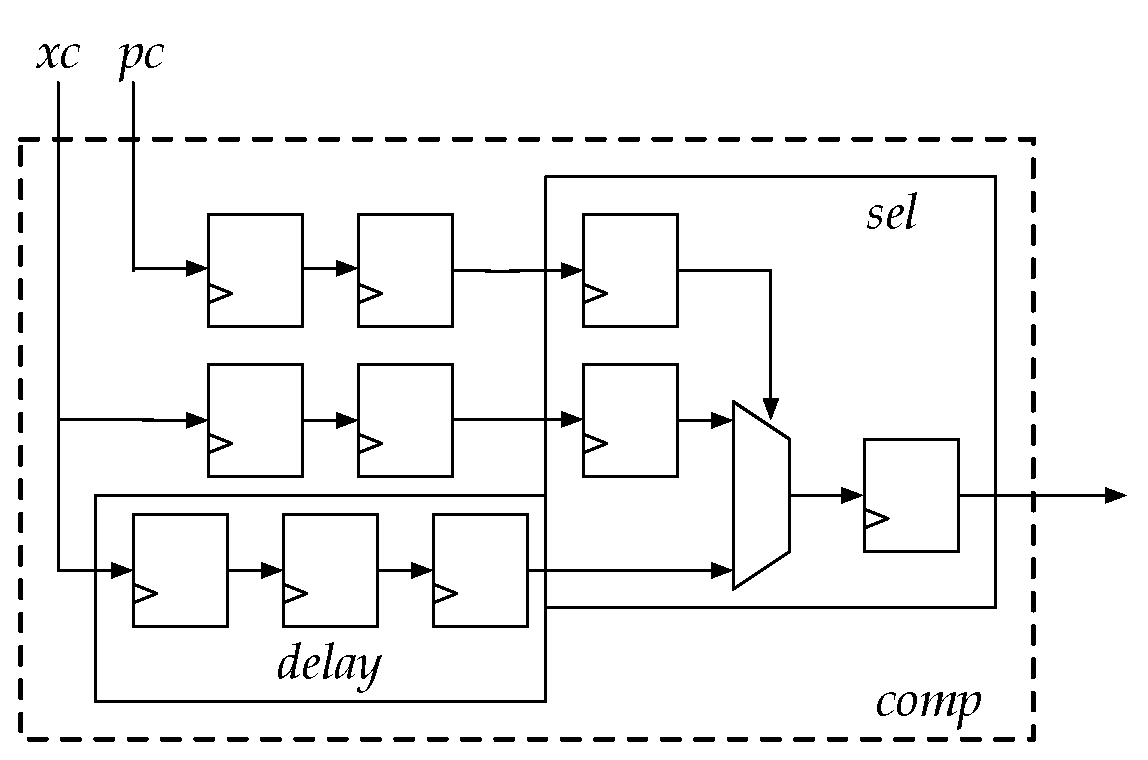
\includegraphics[width=0.8\textwidth]{images/compositionsel}
\end{center}
\caption{Composition of \ensuremath{\Varid{sel}} and \ensuremath{\Varid{delayI}} to create \ensuremath{\Varid{comp}}.} \label{fig:compositionsel}
\end{figure}


The code from code snippet \ref{code:constraintgenex1} is represented by the \gls{ast} of code snippet \ref{code:constraintgenex2}.
The term \ensuremath{\Varid{comp}} is passed to the \ensuremath{\Varid{contraints}} function as explained in the previous section.

\begin{texexptitled}[text only]{Example of constraint generation (2).}{code:constraintgenex2}
\begin{hscode}\SaveRestoreHook
\column{B}{@{}>{\hspre}l<{\hspost}@{}}%
\column{9}{@{}>{\hspre}l<{\hspost}@{}}%
\column{11}{@{}>{\hspre}l<{\hspost}@{}}%
\column{15}{@{}>{\hspre}l<{\hspost}@{}}%
\column{17}{@{}>{\hspre}l<{\hspost}@{}}%
\column{23}{@{}>{\hspre}l<{\hspost}@{}}%
\column{25}{@{}>{\hspre}l<{\hspost}@{}}%
\column{E}{@{}>{\hspre}l<{\hspost}@{}}%
\>[B]{}\Varid{delayI}\mathrel{=}{}\<[11]%
\>[11]{}\Conid{TmTAbs}\;\text{\tt \char34 t0\char34}\mathbin{\$}{}\<[E]%
\\
\>[11]{}\Conid{TmAs}\;{}\<[17]%
\>[17]{}(\Conid{TmAbs}\;\text{\tt \char34 xd\char34}\;(\Conid{TmVar}\;\mathrm{0}))\mathbin{\$}{}\<[E]%
\\
\>[17]{}\Conid{Arrow}\;{}\<[25]%
\>[25]{}(\Conid{Constant}\mathbin{\$}\Conid{TimedType}\;\Conid{TyInt}\;(\Conid{TimeExpr}\;\mathrm{0}\;\mathrm{0}))\;{}\<[E]%
\\
\>[25]{}(\Conid{Constant}\mathbin{\$}\Conid{TimedType}\;\Conid{TyInt}\;(\Conid{TimeExpr}\;\mathrm{0}\;\mathrm{3})){}\<[E]%
\\[\blanklineskip]%
\>[B]{}\Varid{sel}\mathrel{=}{}\<[9]%
\>[9]{}\Conid{TmTAbs}\;\text{\tt \char34 t1\char34}\mathbin{\$}{}\<[E]%
\\
\>[9]{}\Conid{TmAs}\;{}\<[15]%
\>[15]{}(\Conid{TmAbs}\;\text{\tt \char34 p\char34}\mathbin{\$}\Conid{TmAbs}\;\text{\tt \char34 x\char34}\mathbin{\$}\Conid{TmAbs}\;\text{\tt \char34 y\char34}\mathbin{\$}{}\<[E]%
\\
\>[15]{}(\Conid{TmIf}\;(\Conid{TmVar}\;\mathrm{2})\;(\Conid{TmVar}\;\mathrm{1})\;(\Conid{TmVar}\;\mathrm{0})))\;{}\<[E]%
\\
\>[15]{}(\Conid{Arrow}\;{}\<[23]%
\>[23]{}(\Conid{Constant}\mathbin{\$}\Conid{TimedType}\;\Conid{TyBool}\;(\Conid{TimeExpr}\;\mathrm{0}\;\mathrm{0})){}\<[E]%
\\
\>[15]{}(\Conid{Arrow}\;{}\<[23]%
\>[23]{}(\Conid{Constant}\mathbin{\$}\Conid{TimedType}\;\Conid{TyInt}\;(\Conid{TimeExpr}\;\mathrm{0}\;\mathrm{0})){}\<[E]%
\\
\>[15]{}(\Conid{Arrow}\;{}\<[23]%
\>[23]{}(\Conid{Constant}\mathbin{\$}\Conid{TimedType}\;\Conid{TyInt}\;(\Conid{TimeExpr}\;\mathrm{0}\;\mathrm{1}))\;{}\<[E]%
\\
\>[23]{}(\Conid{Constant}\mathbin{\$}\Conid{TimedType}\;\Conid{TyInt}\;(\Conid{TimeExpr}\;\mathrm{0}\;\mathrm{2}))))){}\<[E]%
\\[\blanklineskip]%
\>[B]{}\Varid{comp}\mathrel{=}{}\<[9]%
\>[9]{}\Conid{TmAbs}\;\text{\tt \char34 pc\char34}\mathbin{\$}\Conid{TmAbs}\;\text{\tt \char34 xc\char34}\mathbin{\$}{}\<[E]%
\\
\>[9]{}\Conid{TmApp}\;{}\<[17]%
\>[17]{}(\Conid{TmApp}\;{}\<[25]%
\>[25]{}(\Conid{TmApp}\;\Varid{sel}\;(\Conid{TmVar}\;\mathrm{1}))\;{}\<[E]%
\\
\>[25]{}(\Conid{TmVar}\;\mathrm{0}))\;{}\<[E]%
\\
\>[17]{}(\Conid{TmApp}\;\Varid{delayI}\;(\Conid{TmVar}\;\mathrm{0})){}\<[E]%
\ColumnHook
\end{hscode}\resethooks
\end{texexptitled}

The constraints which are generated by the constraint generation algorithm include many type variables.
We choose to represent type variables by \ensuremath{\Conid{Xn}}, where \ensuremath{\Varid{n}} is the unique identifier for the type variable.
Similarly, we choose to represent the time variables by \ensuremath{\Varid{tn}}.
The constraints generated by the algorithm for \ensuremath{\Varid{comp}} are the following:
\begin{changemargin}{1cm}{0cm}
\begin{expansionno}{text only}
\begin{tabular}{l l}
\ensuremath{\Conid{X1}\mathrel{=}\Conid{X0}\to \Conid{X3}}   &   \ensuremath{\Conid{X3}\mathrel{=}\Conid{X2}\to \Conid{X15}} \\
\ensuremath{\Conid{X7}\mathrel{=}\Conid{Bool}\langle\Varid{t2}\rangle}   &   \ensuremath{\Conid{X13}\mathrel{=}\Conid{X2}\to \Conid{X14}} \\
\ensuremath{\Conid{X8}\mathrel{=}\Conid{X0}\to \Conid{X13}}  &   \ensuremath{\Conid{X8}\mathrel{=}\Conid{Bool}\langle\Varid{t1}\mathbin{+}\mathrm{0}\rangle\to \Conid{Int}\langle\Varid{t1}\mathbin{+}\mathrm{0}\rangle} \\ 
                  &   $\quad\:$ \ensuremath{\to \Conid{Int}\langle\Varid{t1}\mathbin{+}\mathrm{1}\rangle\to \Conid{Int}\langle\Varid{t1}\mathbin{+}\mathrm{2}\rangle} \\
\ensuremath{\Conid{X8}\mathrel{=}\Conid{X7}\to \Conid{X10}}  &   \ensuremath{\Conid{X10}\mathrel{=}\Conid{X9}\to \Conid{X12}} \\
\ensuremath{\Conid{X5}\mathrel{=}\Conid{X2}\to \Conid{X6}}   &   \ensuremath{\Conid{X14}\mathrel{=}\Conid{X6}\to \Conid{X15}}\\
\ensuremath{\Conid{X9}\mathrel{=}\Conid{X11}}        &   \ensuremath{\Conid{X12}\mathrel{=}\Conid{X11}\to \Conid{X9}}\\
\ensuremath{\Conid{X5}\mathrel{=}\Conid{X4}\to \Conid{X4}}   &   \ensuremath{\Conid{X5}\mathrel{=}\Conid{Int}\langle\Varid{t0}\rangle\to \Conid{Int}\langle\Varid{t0}\mathbin{+}\mathrm{3}\rangle}\\
\end{tabular}
\end{expansionno}
\end{changemargin}

As shown, the ascription introduces the constraints \ensuremath{\Conid{X8}\mathrel{=}\Conid{Bool}\langle\Varid{t1}\mathbin{+}\mathrm{0}\rangle\to \Conid{Int}\langle\Varid{t1}\mathbin{+}\mathrm{0}\rangle\to \Conid{Int}\langle\Varid{t1}\mathbin{+}\mathrm{1}\rangle\to \Conid{Int}\langle\Varid{t1}\mathbin{+}\mathrm{2}\rangle} and \ensuremath{\Conid{X5}\mathrel{=}\Conid{Int}\langle\Varid{t0}\rangle\to \Conid{Int}\langle\Varid{t0}\mathbin{+}\mathrm{3}\rangle} for \ensuremath{\Varid{sel}} and \ensuremath{\Varid{delayI}} respectively.
The constraint \ensuremath{\Conid{X7}\mathrel{=}\Conid{Bool}\langle\Varid{t2}\rangle} is introduced by the \ensuremath{\Conid{TmIf}} rule.
To provide a mapping between type variables and types, we must unify the constraints, which we discuss in the next section.

\section{Unification}
We chose to implement a single unification algorithm, which is flexible enough to allow unification of time expressions, as well as unification of base types.
The similarities between both forms of unification are big enough to warrant a flexible definition.
Moreover, at the point of creating the implementation, the method of checking the time expressions was still in development.
As such, a flexible form of unification helped with development, as it allows us to easily modify the unification algorithm.
The unification algorithm is shown by code snippet \ref{code:unification}.
Before applying \ensuremath{\Varid{unify}} to the set of constraints, the constraints are split in a base type part, as well as a part which only contains time expressions.
The unification algorithm only works on constraints which are instances of the \ensuremath{\Conid{Substitutable}} typeclass, shown by code snippet \ref{code:substitutable}.

\begin{texexptitled}[text only]{Substitutable typeclass}{code:substitutable}
\begin{hscode}\SaveRestoreHook
\column{B}{@{}>{\hspre}l<{\hspost}@{}}%
\column{5}{@{}>{\hspre}l<{\hspost}@{}}%
\column{13}{@{}>{\hspre}l<{\hspost}@{}}%
\column{E}{@{}>{\hspre}l<{\hspost}@{}}%
\>[B]{}\mathbf{class}\;\Conid{Eq}\;\Varid{a}\Rightarrow \Conid{Substitutable}\;\Varid{z}\;\Varid{a}\;\mathbf{where}{}\<[E]%
\\
\>[B]{}\hsindent{5}{}\<[5]%
\>[5]{}\Varid{add}{}\<[13]%
\>[13]{}\mathbin{::}\Conid{Substitution}\;\Varid{a}\to \Varid{z}\to \Varid{z}{}\<[E]%
\\
\>[B]{}\hsindent{5}{}\<[5]%
\>[5]{}\Varid{apply}{}\<[13]%
\>[13]{}\mathbin{::}([\mskip1.5mu \Conid{Substitution}\;\Varid{a}\mskip1.5mu]\to [\mskip1.5mu \Conid{Substitution}\;\Varid{a}\mskip1.5mu])\to \Varid{z}\to \Varid{z}{}\<[E]%
\\
\>[B]{}\hsindent{5}{}\<[5]%
\>[5]{}\Varid{match}{}\<[13]%
\>[13]{}\mathbin{::}\Varid{a}\to \Varid{a}\to \Varid{z}\to \Varid{z}{}\<[E]%
\ColumnHook
\end{hscode}\resethooks
\end{texexptitled}

\begin{texexptitled}[text only]{Unification}{code:unification}
\begin{hscode}\SaveRestoreHook
\column{B}{@{}>{\hspre}l<{\hspost}@{}}%
\column{5}{@{}>{\hspre}l<{\hspost}@{}}%
\column{9}{@{}>{\hspre}l<{\hspost}@{}}%
\column{30}{@{}>{\hspre}c<{\hspost}@{}}%
\column{30E}{@{}l@{}}%
\column{33}{@{}>{\hspre}l<{\hspost}@{}}%
\column{39}{@{}>{\hspre}l<{\hspost}@{}}%
\column{43}{@{}>{\hspre}l<{\hspost}@{}}%
\column{47}{@{}>{\hspre}l<{\hspost}@{}}%
\column{49}{@{}>{\hspre}l<{\hspost}@{}}%
\column{55}{@{}>{\hspre}l<{\hspost}@{}}%
\column{E}{@{}>{\hspre}l<{\hspost}@{}}%
\>[B]{}\Varid{unify}\mathbin{::}(\Conid{Show}\;\Varid{a},\Conid{Substitutable}\;\Varid{z}\;\Varid{a})\Rightarrow [\mskip1.5mu \Conid{Constraint}\;\Varid{a}\mskip1.5mu]\to \Varid{z}\to \Varid{z}{}\<[E]%
\\
\>[B]{}\Varid{unify}\;[\mskip1.5mu \mskip1.5mu]\;\Varid{r}\mathrel{=}\Varid{id}\;\Varid{r}{}\<[E]%
\\
\>[B]{}\Varid{unify}\;(\Varid{c}\mathbin{:}\Varid{cs})\;\Varid{r}\mathrel{=}\mathbf{case}\;\Varid{c}\;\mathbf{of}{}\<[E]%
\\
\>[B]{}\hsindent{5}{}\<[5]%
\>[5]{}(\Conid{Constant}\;\Varid{t1},\Conid{Constant}\;\Varid{t2}){}\<[33]%
\>[33]{}\to \Varid{unify}\;\Varid{cs}\mathbin{\$}\Varid{match}\;\Varid{t1}\;\Varid{t2}\;\Varid{r}{}\<[E]%
\\
\>[B]{}\hsindent{5}{}\<[5]%
\>[5]{}(\Conid{Arrow}\;\Varid{s1}\;\Varid{s2},\Conid{Arrow}\;\Varid{t1}\;\Varid{t2}){}\<[39]%
\>[39]{}\to \Varid{unify}\;((\Varid{s1},\Varid{t1})\mathbin{:}(\Varid{s2},\Varid{t2})\mathbin{:}\Varid{cs})\;\Varid{r}{}\<[E]%
\\
\>[B]{}\hsindent{5}{}\<[5]%
\>[5]{}(\Varid{tyS}\mathord{@}(\Conid{Var}\;\Varid{idS}),\Varid{tyT}{}\<[30]%
\>[30]{}){}\<[30E]%
\\
\>[5]{}\hsindent{4}{}\<[9]%
\>[9]{}\mid \Varid{tyS}\equiv \Varid{tyT}{}\<[39]%
\>[39]{}\to {}\<[43]%
\>[43]{}\Varid{unify}\;\Varid{cs}\;\Varid{r}{}\<[E]%
\\
\>[5]{}\hsindent{4}{}\<[9]%
\>[9]{}\mid \neg \mathbin{\$}\Varid{idS}\mathbin{`\Varid{isFVIn}`}\Varid{tyT}{}\<[39]%
\>[39]{}\to {}\<[43]%
\>[43]{}\mathbf{let}\;{}\<[49]%
\>[49]{}\Varid{cs'}{}\<[55]%
\>[55]{}\mathrel{=}(\Varid{tyS}\mapsto\Varid{tyT})\;\Varid{cs}{}\<[E]%
\\
\>[49]{}\Varid{r'}{}\<[55]%
\>[55]{}\mathrel{=}\Varid{add}\;(\Varid{tyS},\Varid{tyT})\mathbin{\$}\Varid{apply}\;(\Varid{tyS}\mapsto\Varid{tyT})\;\Varid{r}{}\<[E]%
\\
\>[43]{}\mathbf{in}\;{}\<[47]%
\>[47]{}\Varid{unify}\;\Varid{cs'}\;\Varid{r'}{}\<[E]%
\\[\blanklineskip]%
\>[B]{}\hsindent{5}{}\<[5]%
\>[5]{}(\Varid{tyS},\Varid{tyT}\mathord{@}(\Conid{Var}\;\Varid{idT}){}\<[30]%
\>[30]{}){}\<[30E]%
\>[39]{}\to \Varid{unify}\;((\Varid{tyT},\Varid{tyS})\mathbin{:}\Varid{cs})\;\Varid{r}{}\<[E]%
\\
\>[B]{}\hsindent{5}{}\<[5]%
\>[5]{}(\Varid{t1},\Varid{t2}{}\<[30]%
\>[30]{}){}\<[30E]%
\>[39]{}\to \Varid{error}\;\text{\tt \char34 not~unifiable~\char34}{}\<[E]%
\ColumnHook
\end{hscode}\resethooks
\end{texexptitled}

In the substitutable typeclass, \ensuremath{\Varid{a}} represents the type of constraints, which is either a base type or a time expression.
Depending on the type of constraints, a different record can be used to build the list of substitutions.
The list of substitutions provides a mapping between type variables and constant types.
The different operations of the \ensuremath{\Conid{Substitutable}} typeclass are explained when we discuss the unification algorithm.
However, we point out that these operations, together with the polymorphic container type \ensuremath{\Varid{z}}, allow us to modify the resulting substitutions by the unification algorithm.

As shown, \ensuremath{\Varid{unify}} accepts two arguments.
One is a set of constraints, the other being a record type which is defined by the \ensuremath{\Conid{Substitutable}} typeclass.
To clarify the algorithm, we first focus on how it is implemented for base types, before showing how it is implemented for time expressions.
The base type instance of the \ensuremath{\Conid{Substitutable}} typeclass is defined by code snippet \ref{code:priminstance}.

\begin{texexptitled}[text only]{BaseTypes instance}{code:priminstance}
\begin{hscode}\SaveRestoreHook
\column{B}{@{}>{\hspre}l<{\hspost}@{}}%
\column{5}{@{}>{\hspre}l<{\hspost}@{}}%
\column{9}{@{}>{\hspre}l<{\hspost}@{}}%
\column{E}{@{}>{\hspre}l<{\hspost}@{}}%
\>[B]{}\mathbf{type}\;\Conid{Substitution}\;\Varid{a}\mathrel{=}(\Conid{MetaType}\;\Varid{a},\Conid{MetaType}\;\Varid{a}){}\<[E]%
\\
\>[B]{}\mathbf{data}\;\Conid{BaseRecord}\mathrel{=}\Conid{BaseRecord}\;[\mskip1.5mu \Conid{Substitution}\;\Conid{BaseType}\mskip1.5mu]{}\<[E]%
\\[\blanklineskip]%
\>[B]{}\mathbf{instance}\;\Conid{Substitutable}\;\Conid{BaseRecord}\;\Conid{BaseType}\;\mathbf{where}{}\<[E]%
\\
\>[B]{}\hsindent{5}{}\<[5]%
\>[5]{}\Varid{add}\;\Varid{x}\;(\Conid{BaseRecord}\;\Varid{xs})\mathrel{=}\Conid{BaseRecord}\;(\Varid{x}\mathbin{:}\Varid{xs}){}\<[E]%
\\
\>[B]{}\hsindent{5}{}\<[5]%
\>[5]{}\Varid{apply}\;\Varid{f}\;(\Conid{BaseRecord}\;\Varid{xs})\mathrel{=}\Conid{BaseRecord}\mathbin{\$}\Varid{f}\;\Varid{xs}{}\<[E]%
\\
\>[B]{}\hsindent{5}{}\<[5]%
\>[5]{}\Varid{match}\;\Varid{x}\;\Varid{y}\;\Varid{tr}{}\<[E]%
\\
\>[5]{}\hsindent{4}{}\<[9]%
\>[9]{}\mid \Varid{x}\equiv \Varid{y}\mathrel{=}\Varid{tr}{}\<[E]%
\\
\>[5]{}\hsindent{4}{}\<[9]%
\>[9]{}\mid \Varid{otherwise}\mathrel{=}\Varid{error}\;\text{\tt \char34 x~/=~y\char34}{}\<[E]%
\ColumnHook
\end{hscode}\resethooks
\end{texexptitled}

The \ensuremath{\Varid{unify}} function has five distinct cases of constraints which are handled.
First, the constraint between two constant types are compared.
For this, the \ensuremath{\Varid{match}} function is used, which is part of the \ensuremath{\Conid{Substitutable}} typeclass. 
The functionality of \ensuremath{\Varid{match}} depends on the type of constraints which are unified.
In the case of base types, \ensuremath{\Varid{match}} just checks for equality.
When base types are not equal, an error is raised to indicate that the checked term is not well-typed.

The second case of \ensuremath{\Varid{unify}} handles function constraints, where a function type is constrained by another function type. 
When a function type is constrained by a non-function type, then the term is not well-typed.
If it is constrained by another function type, the individual types which make up the function types are \textit{added} to the existing set of constraints.

The third case of \ensuremath{\Varid{unify}} matches a type variable $X_{idS}$ to an unknown type \ensuremath{\Varid{tyT}}.
If the left hand side of the constraint is equal to the right hand side, then the constraint is discarded and unification continues for the remaining constraints.
If they are not the same, then it is checked whether or not the type variable $X_{idS}$ exists as a free type variable within $tyT$.
Checking for free type variables are important.  
Consider the constraint \ensuremath{\Conid{X0}\mathrel{=}\Conid{X1}\to \Conid{X0}}, where \ensuremath{\Conid{X0}} is not free in \ensuremath{\Conid{X1}\to \Conid{X0}}.
This constraint is not well-typed, as we do not support recursion.

If this is not the case, then the variable $X_{idS}$ is replaced by \ensuremath{\Varid{tyT}} in the remaining constraints, as indicated by the \ensuremath{(\mapsto)} function.
Since we have made a substitution in the form of $X_{idS} \mapsto tyT$, we store the substitution.
However, aside from applying the substitution to the remaining constraints, the substitution is also applied to the existing substitutions, which is what the \ensuremath{\Varid{apply}} function does in the case of base types.
The way existing substutions are stored depends on the type of constraints which are being unified.
As a result, the functions \ensuremath{\Varid{add}} and \ensuremath{\Varid{apply}} are part of the \ensuremath{\Conid{Substitutable}} typeclass.
In the case of base types, substitutions are added to the record, while existing substitutions within the record are rewritten according to the new substitution.
The fourth case of \ensuremath{\Varid{unify}} is the same as the third case, only with the right hand side and left hand side switched. 
Finally, the fifth case represents the case when terms are not well-typed.

\begin{texexptitled}[text only]{\ensuremath{\Conid{TimeExpr}} instance of \ensuremath{\Conid{Substitutable}}}{code:timeinstance}
\begin{hscode}\SaveRestoreHook
\column{B}{@{}>{\hspre}l<{\hspost}@{}}%
\column{5}{@{}>{\hspre}l<{\hspost}@{}}%
\column{7}{@{}>{\hspre}l<{\hspost}@{}}%
\column{12}{@{}>{\hspre}l<{\hspost}@{}}%
\column{17}{@{}>{\hspre}l<{\hspost}@{}}%
\column{E}{@{}>{\hspre}l<{\hspost}@{}}%
\>[B]{}\mathbf{data}\;\Conid{TimeRecord}\mathrel{=}\Conid{TimeRecord}{}\<[E]%
\\
\>[B]{}\hsindent{17}{}\<[17]%
\>[17]{}\{\mskip1.5mu \Varid{timeSubs}\mathbin{::}[\mskip1.5mu \Conid{Substitution}\;\Conid{TimeExpr}\mskip1.5mu]{}\<[E]%
\\
\>[B]{}\hsindent{17}{}\<[17]%
\>[17]{},\Varid{timeVars}\mathbin{::}[\mskip1.5mu (\Conid{TimeExpr},\Conid{TimeExpr})\mskip1.5mu]\mskip1.5mu\}{}\<[E]%
\\[\blanklineskip]%
\>[B]{}\mathbf{instance}\;\Conid{Substitutable}\;\Conid{TimeRecord}\;\Conid{TimeExpr}\;\mathbf{where}{}\<[E]%
\\
\>[B]{}\hsindent{5}{}\<[5]%
\>[5]{}\Varid{add}\;\Varid{x}\;\Varid{tr}\mathrel{=}\Varid{tr}\;\{\mskip1.5mu \Varid{timeSubs}\mathrel{=}\Varid{x}\mathbin{:}(\Varid{timeSubs}\;\Varid{tr})\mskip1.5mu\}{}\<[E]%
\\
\>[B]{}\hsindent{5}{}\<[5]%
\>[5]{}\Varid{apply}\;\Varid{f}\;\Varid{tr}\mathrel{=}\Varid{tr}\;\{\mskip1.5mu \Varid{timeSubs}\mathrel{=}\Varid{f}\mathbin{\$}\Varid{timeSubs}\;\Varid{tr}\mskip1.5mu\}{}\<[E]%
\\
\>[B]{}\hsindent{5}{}\<[5]%
\>[5]{}\Varid{match}\;\Varid{x}\;\Varid{y}\;\Varid{tr}\mathrel{=}{}\<[E]%
\\
\>[5]{}\hsindent{2}{}\<[7]%
\>[7]{}\mathbf{let}\;\Varid{maysub}\mathrel{=}\Varid{matchConstantType}\;(\Varid{x},\Varid{y}){}\<[E]%
\\
\>[5]{}\hsindent{2}{}\<[7]%
\>[7]{}\mathbf{in}\;\mathbf{case}\;\Varid{maysub}\;\mathbf{of}{}\<[E]%
\\
\>[7]{}\hsindent{5}{}\<[12]%
\>[12]{}\Conid{Just}\;\Varid{z}\to \Varid{tr}\;\{\mskip1.5mu \Varid{timeVars}\mathrel{=}\Varid{z}\mathbin{:}(\Varid{timeVars}\;\Varid{tr})\mskip1.5mu\}{}\<[E]%
\\
\>[7]{}\hsindent{5}{}\<[12]%
\>[12]{}\Conid{Nothing}\to \Varid{tr}{}\<[E]%
\ColumnHook
\end{hscode}\resethooks
\end{texexptitled}

The same algorithm is used for time expressions. 
The code of snippet \ref{code:timeinstance} shows the \ensuremath{\Conid{TimeExpr}} instance of \ensuremath{\Conid{Substitutable}}.
The unification algorithm uses \ensuremath{\Conid{TimeRecord}} to store substitutions.
The \ensuremath{\Varid{timeSubs}} stores the substitutions, while \ensuremath{\Varid{timeVars}} is used to verify time expressions.
To create substitutions, first the unification algorithm finds the relations between time expressions which are needed to verify the time-dependent behaviour.
These relations are stored in \ensuremath{\Varid{timeVars}}.
After the time-expressions are verified, the \textit{original} set of constraints is modified.
The resulting constraints are then unified \textit{again}, after which \ensuremath{\Varid{timeSubs}} contains the final substitutions.
Adding the substitutions and applying them to time variables is straightforward.
However, matching time expressions is more complex, as shown by code snippet \ref{code:timematch}.
The result of \ensuremath{\Varid{matchConstantType}} are added to \ensuremath{\Varid{timeVars}}, which is used to verify the time expressions.

\begin{texexptitled}[text only]{Matching function for time expressions}{code:timematch}
\begin{hscode}\SaveRestoreHook
\column{B}{@{}>{\hspre}l<{\hspost}@{}}%
\column{3}{@{}>{\hspre}l<{\hspost}@{}}%
\column{5}{@{}>{\hspre}l<{\hspost}@{}}%
\column{7}{@{}>{\hspre}l<{\hspost}@{}}%
\column{21}{@{}>{\hspre}l<{\hspost}@{}}%
\column{25}{@{}>{\hspre}l<{\hspost}@{}}%
\column{E}{@{}>{\hspre}l<{\hspost}@{}}%
\>[B]{}\Varid{matchConstantType}\;\Varid{c}\mathrel{=}{}\<[E]%
\\
\>[B]{}\hsindent{3}{}\<[3]%
\>[3]{}\mathbf{case}\;\Varid{c}\;\mathbf{of}{}\<[E]%
\\
\>[3]{}\hsindent{2}{}\<[5]%
\>[5]{}(\Conid{TimeExpr}\;\Varid{t1}\;\Varid{o1},\Conid{TimeExpr}\;\Varid{t2}\;\Varid{o2}){}\<[E]%
\\
\>[5]{}\hsindent{2}{}\<[7]%
\>[7]{}\mid \Varid{t1}\equiv \Varid{t2}{}\<[21]%
\>[21]{}\to {}\<[25]%
\>[25]{}\Conid{Nothing}{}\<[E]%
\\
\>[5]{}\hsindent{2}{}\<[7]%
\>[7]{}\mid \Varid{otherwise}{}\<[21]%
\>[21]{}\to {}\<[25]%
\>[25]{}\Conid{Just}\;(\Conid{TimeExpr}\;\Varid{t1}\;\Varid{o1},\Conid{TimeExpr}\;\Varid{t2}\;\Varid{o2}){}\<[E]%
\\[\blanklineskip]%
\>[3]{}\hsindent{2}{}\<[5]%
\>[5]{}(\Conid{TimeLiteral}\;\Varid{o1},\Conid{TimeLiteral}\;\Varid{o2}){}\<[E]%
\\
\>[5]{}\hsindent{2}{}\<[7]%
\>[7]{}\mid \Varid{o1}\equiv \Varid{o2}{}\<[21]%
\>[21]{}\to {}\<[25]%
\>[25]{}\Conid{Nothing}{}\<[E]%
\\
\>[5]{}\hsindent{2}{}\<[7]%
\>[7]{}\mid \Varid{otherwise}{}\<[21]%
\>[21]{}\to {}\<[25]%
\>[25]{}\Varid{error}\;\text{\tt \char34 cannot~unify~literals~o1~o2\char34}{}\<[E]%
\\[\blanklineskip]%
\>[3]{}\hsindent{2}{}\<[5]%
\>[5]{}(\Varid{c1}\mathord{@}(\Conid{TimeExpr}\;\Varid{t1}\;\Varid{o1}),\Varid{c2}\mathord{@}(\Conid{TimeLiteral}\;\Varid{o2})){}\<[E]%
\\
\>[5]{}\hsindent{16}{}\<[21]%
\>[21]{}\to {}\<[25]%
\>[25]{}\Conid{Just}\;(\Varid{c2},\Varid{c1}){}\<[E]%
\\[\blanklineskip]%
\>[3]{}\hsindent{2}{}\<[5]%
\>[5]{}(\Varid{c1}\mathord{@}(\Conid{TimeLiteral}\;\Varid{o1}),\Varid{c2}\mathord{@}(\Conid{TimeExpr}\;\Varid{t2}\;\Varid{o2})){}\<[E]%
\\
\>[5]{}\hsindent{16}{}\<[21]%
\>[21]{}\to \Varid{matchConstantType}\;\Varid{c2}\;\Varid{c1}{}\<[E]%
\ColumnHook
\end{hscode}\resethooks
\end{texexptitled}

When matching time expressions, four different cases can be distinguished.
Either a time expression is constrained to another time expression, a literal is constrained to another literal, a literal is constrained by a time expression, or vice versa.
The first case filters the time expressions which are needed to verify the time-dependent behaviour.
For instance, when typechecking the function \ensuremath{\Varid{f}\;\Varid{x}\;\Varid{y}\mathrel{=}\Varid{y}} with type \ensuremath{\Conid{Bool}\langle\Varid{t}\rangle\to \Conid{Bool}\langle\Varid{t}\mathbin{+}\mathrm{1}\rangle\to \Conid{Bool}\langle\Varid{t}\mathbin{+}\mathrm{2}\rangle}, the result would be the equality of \ensuremath{\Conid{Bool}\langle\Varid{t}\mathbin{+}\mathrm{1}\rangle\mathrel{=}\Conid{Bool}\langle\Varid{t}\mathbin{+}\mathrm{2}\rangle}.
This equality is created as \ensuremath{\Varid{y}} on the left hand side of the expression has type \ensuremath{\Conid{Bool}\langle\Varid{t}\mathbin{+}\mathrm{1}\rangle}, while \ensuremath{\Varid{y}} on the right hand side of the expressions has type \ensuremath{\Conid{Bool}\langle\Varid{t}\mathbin{+}\mathrm{2}\rangle}.
Since these time variables are the same, we can determine that this is indeed allowed, as function definitions can only have \textit{increasing} delays.
However, in a constraint with different time variables, such as \ensuremath{\Conid{Bool}\langle\Varid{t0}\mathbin{+}\mathrm{1}\rangle\mathrel{=}\Conid{Bool}\langle\Varid{t1}\mathbin{+}\mathrm{2}\rangle}, we cannot determine if this is actually allowed behaviour.
For the purpose of checking the time constraints at a later point, the constraint is recorded and added to \ensuremath{\Varid{timeVars}}, as shown by code snippet \ref{code:timeinstance}.

The second case of \ensuremath{\Varid{matchConstantType}} checks literals. 
In the prototype typechecker, these literals are only compared for equality.
For the purpose of showing that the principle of checking time expressions actually work this is enough, though it could be extended to allow delays on values which exist at a specific time.

The last two cases of \ensuremath{\Varid{matchConstantType}} check time expressions which are constrained to literals, and vice versa.
When time expressions are constrained to literals, the constraint is added with the left hand side containing the literal, and the right hand side containing the time expression.

\subsection{Example of Unification}
Given the constraints generated earlier, repeated below for convenience, we unify them.
We only show the full unification of base types here.
To show unification of time expressions, we first need to generate the time variables which are checked seperately.

\begin{changemargin}{1cm}{0cm}
\begin{expansionno}{text only}
\begin{tabular}{l l}
\ensuremath{\Conid{X1}\mathrel{=}\Conid{X0}\to \Conid{X3}}   &   \ensuremath{\Conid{X3}\mathrel{=}\Conid{X2}\to \Conid{X15}} \\
\ensuremath{\Conid{X7}\mathrel{=}\Conid{Bool}\langle\Varid{t2}\rangle}   &   \ensuremath{\Conid{X13}\mathrel{=}\Conid{X2}\to \Conid{X14}} \\
\ensuremath{\Conid{X8}\mathrel{=}\Conid{X0}\to \Conid{X13}}  &   \ensuremath{\Conid{X8}\mathrel{=}\Conid{Bool}\langle\Varid{t1}\mathbin{+}\mathrm{0}\rangle\to \Conid{Int}\langle\Varid{t1}\mathbin{+}\mathrm{0}\rangle} \\ 
                  &   $\quad\:$ \ensuremath{\to \Conid{Int}\langle\Varid{t1}\mathbin{+}\mathrm{1}\rangle\to \Conid{Int}\langle\Varid{t1}\mathbin{+}\mathrm{2}\rangle} \\
\ensuremath{\Conid{X8}\mathrel{=}\Conid{X7}\to \Conid{X10}}  &   \ensuremath{\Conid{X10}\mathrel{=}\Conid{X9}\to \Conid{X12}} \\
\ensuremath{\Conid{X5}\mathrel{=}\Conid{X2}\to \Conid{X6}}   &   \ensuremath{\Conid{X14}\mathrel{=}\Conid{X6}\to \Conid{X15}}\\
\ensuremath{\Conid{X9}\mathrel{=}\Conid{X11}}        &   \ensuremath{\Conid{X12}\mathrel{=}\Conid{X11}\to \Conid{X9}}\\
\ensuremath{\Conid{X5}\mathrel{=}\Conid{X4}\to \Conid{X4}}   &   \ensuremath{\Conid{X5}\mathrel{=}\Conid{Int}\langle\Varid{t0}\rangle\to \Conid{Int}\langle\Varid{t0}\mathbin{+}\mathrm{10}\rangle}\\
\end{tabular}
\end{expansionno}
\end{changemargin}

After splitting these constraints into base types and time expressions, we can pass them to the unification algorithm.
In the case of base types, the resulting mapping is 
\begin{changemargin}{1cm}{0cm}
\begin{expansionno}{text only}
\begin{tabular}{l l}
\ensuremath{\Conid{X0}\mathrel{=}\Conid{Bool}}               & \ensuremath{\Conid{X1}\mathrel{=}\Conid{Bool}\to \Conid{Int}\to \Conid{Int}} \\
\ensuremath{\Conid{X2}\mathrel{=}\Conid{Int}}                & \ensuremath{\Conid{X3}\mathrel{=}\Conid{Int}\to \Conid{Int}}\\
\ensuremath{\Conid{X4}\mathrel{=}\Conid{Int}}                & \ensuremath{\Conid{X5}\mathrel{=}\Conid{Int}\to \Conid{Int}}\\
\ensuremath{\Conid{X6}\mathrel{=}\Conid{Int}}                & \ensuremath{\Conid{X7}\mathrel{=}\Conid{Bool}}\\
\ensuremath{\Conid{X8}\mathrel{=}\Conid{Bool}\to \Conid{Int}\to \Conid{Int}\to \Conid{Int}} & \ensuremath{\Conid{X9}\mathrel{=}\Conid{Int}}\\
\ensuremath{\Conid{X10}\mathrel{=}\Conid{Int}\to \Conid{Int}\to \Conid{Int}} & \ensuremath{\Conid{X11}\mathrel{=}\Conid{Int}}\\
\ensuremath{\Conid{X12}\mathrel{=}\Conid{Int}\to \Conid{Int}}        & \ensuremath{\Conid{X13}\mathrel{=}\Conid{Int}\to \Conid{Int}\to \Conid{Int}}\\ 
\ensuremath{\Conid{X14}\mathrel{=}\Conid{Int}\to \Conid{Int}}        & \ensuremath{\Conid{X15}\mathrel{=}\Conid{Int}}
\end{tabular}
\end{expansionno}
\end{changemargin}
The constraint generation algorithm defined the type of \ensuremath{\Varid{comp}} to be equal to \ensuremath{\Conid{X1}}.
As shown, the resulting type of \ensuremath{\Varid{comp}} is \ensuremath{\Conid{Bool}\to \Conid{Int}\to \Conid{Int}}, which is as expected.
The remainder of the constraints define the types of each intermediate expression which makes up \ensuremath{\Varid{comp}}.
Given these types, we can reason about the types of every (partial) function and other values.

For time variables this is slightly different, as we have not checked whether time expressions are actually correct yet.
However, \ensuremath{\Varid{timeVars}} result in a list of constraints, which are shown below.
\begin{changemargin}{1cm}{0cm}
\begin{expansionno}{text only}
\begin{tabular}{c}
\ensuremath{\langle\Varid{t1}\mathbin{+}\mathrm{1}\rangle\mathrel{=}\langle\Varid{t0}\mathbin{+}\mathrm{3}\rangle} \\
\ensuremath{\langle\Varid{t1}\rangle\mathrel{=}\langle\Varid{t0}\rangle} \\
\ensuremath{\langle\Varid{t2}\rangle\mathrel{=}\langle\Varid{t1}\rangle} \\
\end{tabular}
\end{expansionno}
\end{changemargin}

These constraints are used to verify the complete time-dependent behaviour of \ensuremath{\Varid{comp}}, and provide placement information for memory elements.
In the next section we will use the constraints listed above.

\section{Checking Time Constraints}
Multiple methods could be used to verify the time-dependent behaviour using the constraints of \ensuremath{\Varid{timeVars}}.
We chose to use first order logic to express the constrained time expressions, and use \gls{smt} solvers to find integer representations for the time variables used in time expressions.
Using the integer representations for time variables we can then rewrite the time expressions of compositions in terms of a single time variable and its offsets. 

We chose to use the Z3\cite{de2008z3} solver, as it is the only \gls{smt} solver which supports unbounded integers.
A complete discussion about \gls{smt} solvers is out of the scope of this thesis.
However, \citeauthor{de2008z3} define \gls{smt} as follows: ``A \gls{smt} problem is a decision problem for logical first order formulas with respect to combinations of background theories such as: arithmetic, bit-vectors, arrays, and uninterpreted functions.``

Since the Z3 solver is not written in Haskell, we use the library \ensuremath{\Conid{\Conid{Data}.SBV}}\cite{sbv} to handle the interfacing with Z3.
\ensuremath{\Conid{\Conid{Data}.SBV}} provides the Haskell language with the \ensuremath{\Conid{Symbolic}} monad, which allows us to create statements in first order logic.
The library then allows us to use the Z3 solver to find integer representations for time variables.
The usage of \gls{smt} solvers in Haskell or other functional languages is not new.
Liquid Types\cite{rondon2008liquid} for instance are used to extend Hindley-Milner type inference using \gls{smt}-solvers.

As an example, we use the constrained time expressions from the previous section to create a statement in first order logic, which is checked by the Z3 solver.
\begin{changemargin}{1cm}{0cm}
\begin{expansionno}{text only}
\begin{tabular}{c}
\ensuremath{\langle\Varid{t1}\mathbin{+}\mathrm{1}\rangle\mathrel{=}\langle\Varid{t0}\mathbin{+}\mathrm{3}\rangle} \\
\ensuremath{\langle\Varid{t1}\rangle\mathrel{=}\langle\Varid{t0}\rangle} \\
\ensuremath{\langle\Varid{t2}\rangle\mathrel{=}\langle\Varid{t1}\rangle} \\
\end{tabular}
\end{expansionno}
\end{changemargin}

First, the proper ordering is determined.
Since time variables are created in order, we know that the time variable \ensuremath{\Varid{t1}} must occur later than \ensuremath{\Varid{t0}}.
Similarly, \ensuremath{\Varid{t2}} must occur later than \ensuremath{\Varid{t1}}.
Using the constrained time expressions from above, we can then define the following statement using first order logic:
\[
  \begin{array}{l l}
    \exists t0. \exists t1. \exists t2. & t1 + 1 \geq t0 + 3\\
                                        & t1 \geq t0 \\
                                        & t2 \geq t1\\
                                        & t0 \geq 0\\
                                        & t1 \geq 0\\
                                        & t2 \geq 0
  \end{array}
  \]

We create this statement by using the \ensuremath{\Conid{\Conid{Data}.SBV}} library, and ask Z3 to find integer representations for \ensuremath{\Varid{t0}}, \ensuremath{\Varid{t1}} and \ensuremath{\Varid{t2}}.
We do this by using the \ensuremath{\Conid{Symbolic}} monad, as shown by code snippet \ref{code:symbolic}.

\begin{texexptitled}[text only]{Using the \ensuremath{\Conid{Symbolic}} monad to create statements in first order logic.}{code:symbolic}
\begin{hscode}\SaveRestoreHook
\column{B}{@{}>{\hspre}l<{\hspost}@{}}%
\column{3}{@{}>{\hspre}l<{\hspost}@{}}%
\column{7}{@{}>{\hspre}l<{\hspost}@{}}%
\column{27}{@{}>{\hspre}l<{\hspost}@{}}%
\column{E}{@{}>{\hspre}l<{\hspost}@{}}%
\>[B]{}\Varid{representation}\mathrel{=}{}\<[E]%
\\
\>[B]{}\hsindent{3}{}\<[3]%
\>[3]{}\mathbf{do}\;{}\<[7]%
\>[7]{}\Varid{t1}\leftarrow\Varid{exists}\;\text{\tt \char34 t0\char34}{}\<[E]%
\\
\>[7]{}\Varid{t2}\leftarrow\Varid{exists}\;\text{\tt \char34 t1\char34}{}\<[E]%
\\
\>[7]{}\Varid{t3}\leftarrow\Varid{exists}\;\text{\tt \char34 t2\char34}{}\<[E]%
\\
\>[7]{}\Varid{constrain}\mathbin{\$}\Varid{t0}{}\<[27]%
\>[27]{}.\geq\mathrm{0}{}\<[E]%
\\
\>[7]{}\Varid{constrain}\mathbin{\$}\Varid{t1}{}\<[27]%
\>[27]{}.\geq\mathrm{0}{}\<[E]%
\\
\>[7]{}\Varid{constrain}\mathbin{\$}\Varid{t2}{}\<[27]%
\>[27]{}.\geq\mathrm{0}{}\<[E]%
\\
\>[7]{}\Varid{constrain}\mathbin{\$}\Varid{t1}\mathbin{+}\mathrm{1}{}\<[27]%
\>[27]{}.\geq\Varid{t0}\mathbin{+}\mathrm{3}{}\<[E]%
\\
\>[7]{}\Varid{constrain}\mathbin{\$}\Varid{t1}{}\<[27]%
\>[27]{}.\geq\Varid{t0}{}\<[E]%
\\
\>[7]{}\Varid{constrain}\mathbin{\$}\Varid{t2}{}\<[27]%
\>[27]{}.\geq\Varid{t1}{}\<[E]%
\\
\>[7]{}\Varid{solve}\;[\mskip1.5mu \mskip1.5mu]{}\<[E]%
\ColumnHook
\end{hscode}\resethooks
\end{texexptitled}

Using the definition of \ensuremath{\Varid{representation}}, we use the \ensuremath{\Varid{sat}} function of \ensuremath{\Conid{\Conid{Data}.SBV}} to ask the Z3 solver to find a integer representation of \ensuremath{\Varid{t0}}, \ensuremath{\Varid{t1}} and \ensuremath{\Varid{t2}}.
In our experience, Z3 automatically finds the minimal integer values, though this is not guaranteed.
In the future, Z3 will also support optimization criteria, allowing us to guarantee the minimal integer values for time variables.
If the time expressions are erroneous, the \ensuremath{\Varid{sat}} function will not return integer representations for \ensuremath{\Varid{t0}}, \ensuremath{\Varid{t1}} and \ensuremath{\Varid{t2}}.

In the case of verifying the behaviour of \ensuremath{\Varid{comp}} however, the \ensuremath{\Varid{sat}} function provides the following integer representations:
\begin{changemargin}{1cm}{0cm}
\begin{expansionno}{text only}
\ensuremath{\Varid{t0}\mathrel{=}\mathrm{0}}\\
\ensuremath{\Varid{t1}\mathrel{=}\mathrm{2}}\\
\ensuremath{\Varid{t2}\mathrel{=}\mathrm{2}}\\
\end{expansionno}
\end{changemargin}

When we assume \ensuremath{\Varid{t}\mathrel{=}\mathrm{0}}, we can rewrite the existing expressions of the original constraints as follows:

\begin{changemargin}{1cm}{0cm}
\begin{expansionno}{text only}
\begin{tabular}{l l}
\ensuremath{\Conid{X1}\mathrel{=}\Conid{X0}\to \Conid{X3}}   &   \ensuremath{\Conid{X3}\mathrel{=}\Conid{X2}\to \Conid{X15}} \\
\ensuremath{\Conid{X7}\mathrel{=}\Conid{Bool}\langle\Varid{t}\mathbin{+}\mathrm{2}\rangle}   &   \ensuremath{\Conid{X13}\mathrel{=}\Conid{X2}\to \Conid{X14}} \\
\ensuremath{\Conid{X8}\mathrel{=}\Conid{X0}\to \Conid{X13}}  &   \ensuremath{\Conid{X8}\mathrel{=}\Conid{Bool}\langle\Varid{t}\mathbin{+}\mathrm{2}\rangle\to \Conid{Int}\langle\Varid{t}\mathbin{+}\mathrm{2}\rangle} \\ 
                  &   $\quad\:$ \ensuremath{\to \Conid{Int}\langle\Varid{t}\mathbin{+}\mathrm{3}\rangle\to \Conid{Int}\langle\Varid{t}\mathbin{+}\mathrm{4}\rangle} \\
\ensuremath{\Conid{X8}\mathrel{=}\Conid{X7}\to \Conid{X10}}  &   \ensuremath{\Conid{X10}\mathrel{=}\Conid{X9}\to \Conid{X12}} \\
\ensuremath{\Conid{X5}\mathrel{=}\Conid{X2}\to \Conid{X6}}   &   \ensuremath{\Conid{X14}\mathrel{=}\Conid{X6}\to \Conid{X15}}\\
\ensuremath{\Conid{X9}\mathrel{=}\Conid{X11}}        &   \ensuremath{\Conid{X12}\mathrel{=}\Conid{X11}\to \Conid{X9}}\\
\ensuremath{\Conid{X5}\mathrel{=}\Conid{X4}\to \Conid{X4}}   &   \ensuremath{\Conid{X5}\mathrel{=}\Conid{Int}\langle\Varid{t}\rangle\to \Conid{Int}\langle\Varid{t}\mathbin{+}\mathrm{3}\rangle}\\
\end{tabular}
\end{expansionno}
\end{changemargin}

We can then use unification to generate the substitutions for time expressions.
As a result, the following substitutions are created:

\begin{changemargin}{1cm}{0cm}
\begin{expansionno}{text only}
\begin{tabular}{l l}
\ensuremath{\Conid{X0}\mathrel{=}\langle\Varid{t}\mathbin{+}\mathrm{2}\rangle}      &   \ensuremath{\Conid{X1}\mathrel{=}\langle\Varid{t}\mathbin{+}\mathrm{2}\rangle\to \langle\Varid{t}\mathbin{+}\mathrm{2}\rangle\to \langle\Varid{t}\mathbin{+}\mathrm{4}\rangle} \\
\ensuremath{\Conid{X2}\mathrel{=}\langle\Varid{t}\mathbin{+}\mathrm{2}\rangle}      &   \ensuremath{\Conid{X3}\mathrel{=}\langle\Varid{t}\mathbin{+}\mathrm{2}\rangle\to \langle\Varid{t}\mathbin{+}\mathrm{4}\rangle} \\
\ensuremath{\Conid{X4}\mathrel{=}\langle\Varid{t}\mathbin{+}\mathrm{2}\rangle}      &   \ensuremath{\Conid{X5}\mathrel{=}\langle\Varid{t}\mathbin{+}\mathrm{2}\rangle\to \langle\Varid{t}\mathbin{+}\mathrm{3}\rangle} \\ 
\ensuremath{\Conid{X6}\mathrel{=}\langle\Varid{t}\mathbin{+}\mathrm{3}\rangle}      &   \ensuremath{\Conid{X7}\mathrel{=}\langle\Varid{t}\mathbin{+}\mathrm{2}\rangle} \\
\ensuremath{\Conid{X8}\mathrel{=}\langle\Varid{t}\mathbin{+}\mathrm{2}\rangle\to \langle\Varid{t}\mathbin{+}\mathrm{2}\rangle}   &   \ensuremath{\Conid{X9}\mathrel{=}\langle\Varid{t}\mathbin{+}\mathrm{2}\rangle}\\
$\quad \:$ \ensuremath{\to \langle\Varid{t}\mathbin{+}\mathrm{3}\rangle\to \langle\Varid{t}\mathbin{+}\mathrm{4}\rangle} \\
\ensuremath{\Conid{X10}\mathrel{=}\langle\Varid{t}\mathbin{+}\mathrm{2}\rangle\to \langle\Varid{t}\mathbin{+}\mathrm{3}\rangle\to \langle\Varid{t}\mathbin{+}\mathrm{4}\rangle}        &   \ensuremath{\Conid{X11}\mathrel{=}\langle\Varid{t}\mathbin{+}\mathrm{3}\rangle}\\
\ensuremath{\Conid{X12}\mathrel{=}\langle\Varid{t}\mathbin{+}\mathrm{3}\rangle\to \langle\Varid{t}\mathbin{+}\mathrm{4}\rangle}   &   \ensuremath{\Conid{X13}\mathrel{=}\langle\Varid{t}\mathbin{+}\mathrm{2}\rangle\to \langle\Varid{t}\mathbin{+}\mathrm{3}\rangle\to \langle\Varid{t}\mathbin{+}\mathrm{4}\rangle}\\
\ensuremath{\Conid{X14}\mathrel{=}\langle\Varid{t}\mathbin{+}\mathrm{3}\rangle\to \langle\Varid{t}\mathbin{+}\mathrm{4}\rangle}   &   \ensuremath{\Conid{X15}\mathrel{=}\langle\Varid{t}\mathbin{+}\mathrm{4}\rangle}\\
\end{tabular}
\end{expansionno}
\end{changemargin}

The type of the \ensuremath{\Varid{comp}} function, after we combine the above substitution with the base type substitutions, is defined to be \ensuremath{\Conid{X1}\mathrel{=}\Conid{Bool}\langle\Varid{t}\mathbin{+}\mathrm{2}\rangle\to \Conid{Int}\langle\Varid{t}\mathbin{+}\mathrm{2}\rangle\to \Conid{Int}\langle\Varid{t}\mathbin{+}\mathrm{4}\rangle}, which reflects the time-dependent behaviour of \ensuremath{\Varid{comp}}.
As mentioned before, we use flexible composition, and as such the type of \ensuremath{\Varid{comp}} reflects the described circuit of figure \ref{fig:compositionsel} on page \pageref{fig:compositionsel}.

Since all substitutions are written in terms of a single time variable, all time-dependent behaviour from every expression is known.
Since all time-dependent behaviour from every expressions is known, it should \textit{in principle} be possible to derive a circuit description from the type information.

\section{Conclusion}
Even though the implementation is not complete, we have shown that verification and inference of time-dependent behaviour is feasible.
The implementation is not as elegant as it could be however.
Since the implementation was mainly used as a tool to figure out how to verify and infer time-dependent behaviour, it was created without a detailled plan.

If a real implementation were to be made, the usage of \gls{smt}-solvers may not be needed.
While \gls{smt}-solvers allow us to define statements of first order logic, solving these statements does come at a cost.
The computational complexity of \gls{smt}-solvers is known to be non-polynomical, which might make them less suited for larger projects.
Moreover, since the constraints on time expressions are fairly simple, other methods could be used to check the types of expressions and determine register placement. 

The implementation shown here differs from the type system of chapter \ref{ch:typesystem} in a few aspects.
First, the implementation does not use a $\delta$ function to only allow construction of functions which include monotonic increase of delays.
As such, the given implementation might not be as robust as the type system presented earlier.
Instead, ascription is used to bind a type to a term.

Furthermore, in the type system of chapter \ref{ch:typesystem}, we do not use type variables, nor unification.
These are artifacts from adopting Pierce's algorithm, and not strictly needed for an implementation.
In addition, time variables are introduced through a separate term.
In the type system introduced earlier, time variables are scoped using universal and existential quantification as part of either constraints or polytemporal types.


%\section{Introduction}
%For the actual implementation I use DeBruijn indices, primarily so I do not have to deal with scoping problems while developing the timing extensions.
%This will of course make the parsing more complex, but seeing as parsing haskell-esque source code has been done before I hope this will prove only a small burden.
%Internally I simply represent DeBruijn indices as:
%\begin{code}
%type DeBruijn = Int
%\end{code}
%I use DeBruijn indices for a number of things:
%\begin{itemize}
%\item Refering a variable to its binder.
%\item Refering a time variable to its time quantifier.
%\item Refering a variables in a let expression to its definition.
%\end{itemize}
%
%Before going into further details I will first show how I deal with typechecking and checking the timing information.
%To show how the type checker is implemented the following picture shows the different steps in the typechecking process.
%Note that I currently do not have implemented the parsing part.
%\begin{figure}[H]
%\begin{tikzpicture}[scale=0.85,transform shape]
%
%  \path \blocktitle{1}{Parser}{};
%  \path (p1.south)+(0.0,-1.5)   \blocktitle{2}{Constraint generation}{Given a certain term, generate a list of constraints which need to hold in order for the term to have a type};
%  \path (p2.south)+(0.0,-1.5)   \blocktitle{3}{Split}{Splitting base types from timing information};
%  \path (p3.south)+(-3.5,-1.8)  \blocktitle{4}{Unification}{Unifies the constraints of base types, resulting in a mapping of type variables to types.};
%  \path (p3.south)+(3.5,-1.8)   \blocktitle{5}{Unification}{Unifies the constraints of timing information, resulting in a mapping of type variables to concrete time information and time constraints};
%  \path (p5.south)+(0,-1.5)     \blocktitle{6}{Timechecking}{Verifies the timing constraints};
%  \path (p6.south)+(-3.5,-1.5)  \blocktitle{7}{Merge}{Merges timing information with base types, possibly indicating errors if there is a mismatch};
%  \path [line] (p1.south) -- node [above] {} (p2) ;
%  \path [line] (p2.south) -- node [above] {} (p3) ;
%  \path [line] (p3.south) -- +(0.0,-0.5) -- +(-3.5,-0.5)
%    -- node [above, midway] {} (p4);
%  \path [line] (p3.south) -- +(0.0,-0.5) -- +(3.5,-0.5)
%    -- node [above, midway] {} (p5);
%  \path [line] (p5.south) -- node [above] {} (p6) ;
%  \path [line] (p6.south) -- +(0.0,-0.5) -- +(-3.5,-0.5)
%    -- node [above, midway] {} (p7);
% \path [line] (p4.south) -- +(0.0,-2.75) -- +(+3.5,-2.75)
%    -- node [above, midway] {} (p7);
%\end{tikzpicture}
%\end{figure}
%As seen in the flowchart, the entire typechecking part is split in two parts.
%The checking of timing is independent from regular typechecking.
%This approach has some advantages:
%\begin{itemize}
%\item Regular typechecking can be used on the base types, something which is well understood already.
%\item When merging the results from type and timechecking we can verify that the results from timechecking have the same structure as the ones from typechecking.
%      This provides a simple error detection method, increasing the confidence in correctness.
%\item If the timechecking algorithm is independent of typechecking the same approach may be used to augment other typecheckers with time information.
%\item Extending the timechecking part is easier.
%\end{itemize}
%
%Before explaining the details, I will first explain some basic abstraction mechanism, as unification is used more than once.
%To allow this the general structure of types has to be shared between timing information and base types.
%This can be done using a parameterized data type:
%\begin{code}
%type VariableIndex = Int
%
%data MetaType a     =   Arrow (MetaType a) (MetaType a)
%                    |   Var VariableIndex
%                    |   Concrete a
%\end{code}
%, with |VariableIndex| being a unique identifier used for type inference.
%
%We can then then easily split and combine base type information with timing information through a datatype:
%\begin{code}
%data Type   = Type BaseType TimeType
%            deriving (Eq,Show)
%
%data BaseType  =   TyBool
%                    |   TyInt
%                    deriving (Eq,Show)
%
%data TimedType  =   TimeBound TimeVariableIndex Offset
%                |   TimeLiteral Offset
%                |   TimeVar DeBruijn Offset
%                deriving (Eq,Show)
%\end{code}
%The |TimeType| can take on three different forms.
%The |TimeVar| constructor is only used in ascriptions. 
%Using a DeBruijn index it refers to a certain time quantifier ($\psi$ in the grammar)
%
%When generating the constraints this is transformed to the |TimeBound| form, using a unique variable indentifier.
%The last form is a literal, allowing concrete timing information in types.
%
%Since we are now able to easily go from one representation to another (merging and splitting) we can almost define a general implementation for unification.
%However, unification applied to |TimeType| is slightly different than |BaseType|.
%With |BaseType| when a constraint |Concrete x = Concrete y|, with $y$ and $x$ being |BaseType|, is unified the constraint is either thrown away when they are equal, or a type error occurs when they are not the same.
%For |TimeType| this is different however, as we cannot determine from a single constraint if the constraint actually holds.
%For instance, if we have the constraint $N_1 = N_2 + 1$, with $N_x$ being time variables, then we cannot know, just from this information, if the timing is correct.
%
%Before diving into the modification of the unification algorithm I will first determine a method how we can in fact figure out if timing is correct.
%The naive implementation would simply replace timevariables with literals when it encounters them.
%The problem with this approach is that we cannot distinguish anymore between a valid delay (introduced through ascription and bound to a function) or incorrect timing behaviour.
%Say for instance we have a function 
%\begin{code}
%foo :: Bool<n> -> Bool<n+1> -> Bool<n+2>
%foo _ y = y
%\end{code}
%When applied to a value with type |Bool<0>|, we can determine $n = 0$ and subsequently replace $n$ with $0$ in the constraints.
%The problem is, the resulting type as introduced with ascription should be |Bool<2>|, which is not the same as |y :: Bool<1>|. 
%We will run into the comparison of |Bool<1> = Bool <2>| at one point, which in this case is a valid delay.
%However, since we removed all time quantifiers we do not know anymore whether this was a legitimate time delay introduced by ascription, or an error.
%
%Instead, to deal with this problem I first started simply noting constraints.
%When a certain time quantifier is bound to a literal, instead of replacing the time variable with the literal, I replace the literal with the time variable and note the constraint.
%That way the information we need is conserved, as we need to distinguish between legitimate time delays within a function definition and actual type errors.
%There are basically three scenarios we can encounter when comparing time variables:
%\begin{itemize}
%\item A literal is compared to another literal. We can simply compare and error when they are not equal.
%\item A literal compared to a time variable. We can record the constraint and replace all literals with that specific time variable.
%\item A time variable compared to another time variable. This has two distinct scenarios: either the variables are equal (but offsets are not), or they are not equal. 
%      The first situation we can simply ignore, since delays are allowed within a function.
%      The second however, we can't ignore since no delays are allowed when composing functions.
%\end{itemize}
%
%There is a unforseen \todo{Ik ben hier net gister achtergekomen} problem with this approach however.
%Consider the following function:
%
%\begin{code}
%f :: Bool<n> -> Bool<n+1> -> Bool<n+4>
%g :: Bool<m> -> Bool<m+2> -> Bool<m+3>
%
%h   =   let     b   = True :: Bool<0>
%                g'  = g b
%                f'  = f b
%        in      \x -> g' (f' x)
%\end{code}
%, which will typecheck and have type |Bool<1> -> Bool<3>|, which is obviously wrong.
%This happens since, whenever we encounter a literal, all literals are bound to the same time variable.
%The types of |f'| after the substitution |m = 0| is made makes clear what is going on:
%\begin{code}
%f' :: Bool<m+1> -> Bool<m+4>
%g' :: Bool<m+2> -> Bool<m+3>
%\end{code}
%
%From the code it is clear that |f'|s resulting type cannot be used for |g'|, yet since we allow comparisons between two time variables to have different offsets this gives a wrong result.
%It could probably be determined if it is a real delay or a bad type from the ordering in the constraint (e.g. m+4 = m+2 vs m+2 = m+4).
%But since it is pretty clearly meant as an equivalence relation I do not want to depend on the order of constraints. 
%It would probably introduce bugs as well since it is hard to guarantee a certain order without letting go of the simple one to one relation used in constraints.
%
%Instead of rewriting substitutions and constraints to allow for introducing delays at the typelevel I chose to use a different approach.
%The principle is the same as before, however, when comparing time variables with literals and other time variables I chose to simply note the constraint and not do any rewriting.
%This results in both a set of substitutions, and a set of timing constraints. 
%The timing constraints can be checked independently, resulting in a mapping between time variables and actual time moments.\footnote{Het probleem van het detecteren van een delay is nog niet weg, echter omdat we nu wel exact onderscheid kunnen maken tussen verschillende tijdsvariabelen is het mogelijk om het wel te detecteren}
%These can then be substituted in the set of substitutions, resulting in a complete type. 
%
%\subsection{Unification}
%As mentioned by above, the actual unification algorithm is the same, except when |Concrete| types are compared.
%To facilitate this I have defined a typeclass which allows this comparison to be different, together with an abstract mechanism to store possible results from this comparison:
%\begin{code}
%type Substitution a = (MetaType a, MetaType a)
%
%data BaseRecord = BaseRecord [Substitution BaseType]
%
%data TimeRecord         =       TimeRecord 
%                        { timeSubs :: [Substitution TimeType]
%                        , timeVars :: [(TimeType,TimeType)] 
%                        }
%
%class Eq a => Substitutable z a where
%    add :: Substitution a -> z -> z
%    apply :: ([Substitution a] -> [Substitution a]) -> z -> z 
%    match :: MetaType a -> MetaType a -> z -> z 
%
%instance Substitutable TimeRecord TimeType where
%    add x tr = tr { timeSubs = x : (timeSubs tr) }
%    apply f tr = tr { timeSubs = f $ timeSubs tr }
%    match = ... -- left out on purpose
%
%instance Substitutable BaseRecord BaseType where
%    add x (BaseRecord xs) = BaseRecord (x:xs)
%    apply f (BaseRecord xs) = BaseRecord $ f xs
%    match (Concrete x) (Concrete y) tr
%        | x == y = tr
%        | otherwise = error "x /= y"
%\end{code}
%
%These functions are fairly straightforward.
%|add| adds a substitution to a data structure.
%|apply| applies a certain transformation of substitutions to the data structure
%|match| matches two Concrete types and possibly updates a data structure which holds relevant data.
%
%The unification algorithm can then be used for both base types and timing information:
%\begin{code}
%unify :: (Substitutable z a) => [Constraint a] -> z -> z
%unify [] r = id r
%unify (c:cs) r = case c of
%    (Concrete t1, Concrete t2)      -> unify cs $ match (Concrete t1) (Concrete t2) r
%    (Arrow s1 s2, Arrow t1 t2)      -> unify ((s1,t1) : (s2,t2) : cs) r
%    (tyS@(Var idS), tyT      )
%        | tyS == tyT                ->  unify cs r
%        | not $ idS `isFVIn` tyT    ->  let     cs' = (tyS |-> tyT) cs
%                                                r'  = add (tyS,tyT) $ apply (tyS |-> tyT) r
%                                        in      unify cs' r'
%
%    (tyS, tyT@(Var idT)      )      -> unify ((tyT,tyS) : cs) r
%    (t1,t2                   )      -> error "not unifiable "
%\end{code}
